% !TeX program = xelatex
% !TeX encoding = UTF-8
\documentclass[12pt,openany,oneside]{book}

% -----------------------------------------------------------------------------
% Page, mathematics, tables, graphics
% -----------------------------------------------------------------------------
\usepackage[a4paper,top=23mm,bottom=25mm,left=25mm,right=25mm,headheight=17pt]{geometry}
\usepackage{amsmath,amssymb,amsfonts,mathtools,bm}
\usepackage{amsthm}
\usepackage{booktabs,longtable,array,multirow,tabularx}
\usepackage{graphicx}
\graphicspath{{figures/}}
\usepackage{xcolor}
\usepackage{tikz}
\usetikzlibrary{arrows.meta,positioning,calc,fit,shapes.geometric,decorations.pathreplacing,matrix,patterns,3d}
\usepackage[most]{tcolorbox}
\usepackage{enumitem}
\usepackage{listings}
\usepackage{caption}
\usepackage{subcaption}
\usepackage{float}
\usepackage{fancyhdr}
\usepackage{titlesec}
\usepackage{setspace}
\usepackage{microtype}
\usepackage{hyperref}
\usepackage{xepersian}

% -----------------------------------------------------------------------------
% Robust font configuration: same convention as Chapters 4--7
% -----------------------------------------------------------------------------
\IfFontExistsTF{Amiri}
  {\settextfont[Scale=1.08]{Amiri}\setdigitfont{Amiri}}
  {\settextfont[Scale=1.05]{Noto Naskh Arabic}\setdigitfont{Noto Naskh Arabic}}
\IfFontExistsTF{DejaVu Serif}
  {\setlatintextfont{DejaVu Serif}}
  {\setlatintextfont{Latin Modern Roman}}
\IfFontExistsTF{DejaVu Sans Mono}
  {\setmonofont{DejaVu Sans Mono}}
  {\setmonofont{Latin Modern Mono}}

% -----------------------------------------------------------------------------
% Visual identity
% -----------------------------------------------------------------------------
\definecolor{DeepBlue}{HTML}{163A5F}
\definecolor{Accent}{HTML}{B34B35}
\definecolor{SoftBlue}{HTML}{EAF2F8}
\definecolor{SoftGold}{HTML}{FFF6DF}
\definecolor{SoftGreen}{HTML}{EAF7EF}
\definecolor{SoftRed}{HTML}{FCEDEC}
\definecolor{SoftGray}{HTML}{F4F5F6}
\definecolor{CodeGray}{HTML}{F7F7F7}

\hypersetup{
  colorlinks=true,
  linkcolor=DeepBlue,
  citecolor=Accent,
  urlcolor=Accent,
  pdftitle={پردازش تصویر در دهه آینده ـ فصل هشتم: قطعه‌بندی تصویر},
  pdfauthor={جزوه درس کارشناسی ارشد}
}

\setstretch{1.22}
\setlength{\parskip}{0.35em}
\setlength{\parindent}{1.3em}
\setlist[itemize]{itemsep=0.25em,topsep=0.35em,leftmargin=9mm}
\setlist[enumerate]{itemsep=0.25em,topsep=0.35em,leftmargin=10mm}

\pagestyle{fancy}
\fancyhf{}
\fancyhead[R]{\small\thepage}
\fancyhead[L]{\small\nouppercase{\leftmark}}
\renewcommand{\headrulewidth}{0.4pt}

\titleformat{\chapter}[display]
  {\normalfont\huge\bfseries\color{DeepBlue}}
  {\filleft\Large فصل \thechapter}
  {8pt}
  {\filright}
\titleformat{\section}{\Large\bfseries\color{DeepBlue}}{\thesection}{0.7em}{}
\titleformat{\subsection}{\large\bfseries\color{Accent}}{\thesubsection}{0.7em}{}
\titleformat{\subsubsection}{\normalsize\bfseries\color{DeepBlue}}{\thesubsubsection}{0.7em}{}

% -----------------------------------------------------------------------------
% Theorems and boxes
% -----------------------------------------------------------------------------
\newtheorem{definition}{تعریف}[chapter]
\newtheorem{theorem}{قضیه}[chapter]
\newtheorem{proposition}{گزاره}[chapter]
\newtheorem{lemma}{لم}[chapter]
\newtheorem{example}{مثال}[chapter]
\newtheorem{remark}{نکته}[chapter]
\newtheorem{corollary}{نتیجه}[chapter]
\renewcommand{\proofname}{اثبات}

\newtcolorbox{learningbox}{colback=SoftBlue,colframe=DeepBlue,title=اهداف یادگیری,fonttitle=\bfseries,breakable,enhanced}
\newtcolorbox{keybox}[1][]{colback=SoftGold,colframe=Accent,title={#1},fonttitle=\bfseries,breakable,enhanced}
\newtcolorbox{futurebox}{colback=SoftGreen,colframe=green!50!black,title=پل به دهه آینده,fonttitle=\bfseries,breakable,enhanced}
\newtcolorbox{warningbox}{colback=SoftRed,colframe=red!65!black,title=خطای رایج,fonttitle=\bfseries,breakable,enhanced}
\newtcolorbox{workshopbox}[1][]{colback=SoftGray,colframe=black!55,title={کارگاه کد و آزمایش: #1},fonttitle=\bfseries,breakable,enhanced}
\newtcolorbox{researchbox}[1][]{colback=white,colframe=purple!65!black,title={خواندن مقاله و استاندارد: #1},fonttitle=\bfseries,breakable,enhanced}
\newtcolorbox{videobox}{colback=white,colframe=DeepBlue,title=تقسیم پیشنهادی ویدئوهای ۱۵ دقیقه‌ای,fonttitle=\bfseries,breakable,enhanced}
\newtcolorbox{proofbox}[1][]{colback=white,colframe=DeepBlue!65,title={مسیر اثبات: #1},fonttitle=\bfseries,breakable,enhanced}
\newtcolorbox{codecontract}{colback=SoftBlue,colframe=Accent,title=قرارداد میان ریاضیات و کد,fonttitle=\bfseries,breakable,enhanced}
\newtcolorbox{summarybox}{colback=SoftBlue,colframe=DeepBlue,title=جمع‌بندی فصل,fonttitle=\bfseries,breakable,enhanced}
\newtcolorbox{goalbox}{colback=SoftBlue,colframe=DeepBlue,title=هدف فصل,fonttitle=\bfseries,breakable,enhanced}
\newtcolorbox{principlebox}{colback=SoftGold,colframe=Accent,title=اصل راهنما,fonttitle=\bfseries,breakable,enhanced}
\newtcolorbox{algorithmbox}[1]{colback=SoftGray,colframe=DeepBlue,title={#1},fonttitle=\bfseries,breakable,enhanced}
\newtcolorbox{theorembox}[1]{colback=white,colframe=purple!65!black,title={#1},fonttitle=\bfseries,breakable,enhanced}
\newtcolorbox{applicationbox}[1][]{colback=SoftGreen,colframe=green!45!black,title={کاربرد مهندسی: #1},fonttitle=\bfseries,breakable,enhanced}

% -----------------------------------------------------------------------------
% Mathematical notation
% -----------------------------------------------------------------------------
\newcommand{\R}{\mathbb{R}}
\newcommand{\C}{\mathbb{C}}
\newcommand{\N}{\mathbb{N}}
\newcommand{\Z}{\mathbb{Z}}
\newcommand{\Pj}{\mathbb{P}}
\newcommand{\E}{\mathbb{E}}
\newcommand{\Var}{\operatorname{Var}}
\newcommand{\Cov}{\operatorname{Cov}}
\newcommand{\Prob}{\mathbb{P}}
\newcommand{\norm}[1]{\left\lVert #1\right\rVert}
\newcommand{\abs}[1]{\left\lvert #1\right\rvert}
\newcommand{\inner}[2]{\left\langle #1,#2\right\rangle}
\newcommand{\trans}{^{\mathsf T}}
\newcommand{\herm}{^{\mathsf H}}
\newcommand{\inv}{^{-1}}
\newcommand{\vect}[1]{\bm{#1}}
\newcommand{\mat}[1]{\bm{#1}}
\newcommand{\op}[1]{\mathcal{#1}}
\newcommand{\argmin}{\operatorname*{arg\,min}}
\newcommand{\argmax}{\operatorname*{arg\,max}}
\newcommand{\trace}{\operatorname{tr}}
\newcommand{\diag}{\operatorname{diag}}
\newcommand{\rank}{\operatorname{rank}}
\newcommand{\softmax}{\operatorname{softmax}}
\newcommand{\sigmoid}{\operatorname{sigmoid}}
\newcommand{\IoU}{\operatorname{IoU}}
\newcommand{\Dice}{\operatorname{Dice}}
\newcommand{\CE}{\operatorname{CE}}
\newcommand{\KL}{\operatorname{KL}}
\newcommand{\TV}{\operatorname{TV}}
\newcommand{\dist}{\operatorname{dist}}
\newcommand{\diam}{\operatorname{diam}}
\newcommand{\boundary}{\partial}
\newcommand{\ind}{\mathbf 1}
\newcommand{\Lap}{\mat L}

\lstset{
  language=Python,
  basicstyle=\small\ttfamily\color{black},
  columns=fullflexible,
  keepspaces=true,
  backgroundcolor=\color{CodeGray},
  frame=single,
  rulecolor=\color{black!25},
  numbers=left,
  numberstyle=\tiny,
  breaklines=true,
  showstringspaces=false,
  keywordstyle=\bfseries\color{DeepBlue},
  commentstyle=\itshape\color{black!65},
  stringstyle=\color{Accent},
  tabsize=4
}

\begin{document}

% =============================================================================
% Title page
% =============================================================================
\begin{titlepage}
\centering
\vspace*{0.9cm}
{\color{DeepBlue}\rule{0.9\textwidth}{1.1pt}}\\[1.0cm]
{\Huge\bfseries پردازش تصویر در دهه آینده\\[0.3cm]}
{\LARGE\bfseries از عمق ریاضیات تا مهندس حرفه‌ای\\[0.85cm]}
{\Large کتاب ـ جزوه درس کارشناسی ارشد و آزمایشگاه پژوهش‌محور\\[1.1cm]}

\begin{tikzpicture}[node distance=8mm]
\node[draw=DeepBlue,very thick,rounded corners=3mm,fill=SoftBlue,
      minimum width=13.1cm,minimum height=4.8cm,text width=12.6cm,align=center] (a)
{\Large\bfseries فصل هشتم\\[2mm]
\large قطعه‌بندی تصویر و استخراج ناحیه\\[1mm]
\normalsize از آستانه‌گذاری، رشد ناحیه و مدل‌های آماری تا انرژی‌های گرافی،
منحنی‌های فعال، شبکه‌های عمیق و مدل‌های بنیادین قطعه‌بندی};
\node[below=7mm of a,align=center,text width=12.8cm] {
قطعه‌بندی نقطه‌ای است که پردازش تصویر از «تغییر مقدار پیکسل» به «تصمیم درباره ساختار، شیء و معنا» می‌رسد.
این فصل روش‌های کلاسیک و مدرن را با یک زبان مشترک تصمیم، انرژی، احتمال و بهینه‌سازی پیوند می‌دهد.};
\end{tikzpicture}

\vfill
{\large نسخه تفصیلی درس ـ تابستان ۱۴۰۵ / ۲۰۲۶}\\[0.4cm]
{\normalsize قابل کامپایل با \lr{TeX Live + TeXstudio + XeLaTeX}}\\[0.8cm]
{\color{DeepBlue}\rule{0.9\textwidth}{1.1pt}}
\end{titlepage}

\frontmatter

\chapter*{یادداشت روش‌شناختی فصل هشتم}
\addcontentsline{toc}{chapter}{یادداشت روش‌شناختی فصل هشتم}
قطعه‌بندی یکی از کاربردی‌ترین و در عین حال بدتعریف‌ترین مسائل پردازش تصویر است. «قطعه درست» تنها از مقادیر
خاکستری به دست نمی‌آید؛ تعریف آن به هدف، مقیاس، دانش دامنه، نوع برچسب و هزینه خطا بستگی دارد. مرز تومور برای
برنامه‌ریزی جراحی، ناحیه جاده برای ربات، حروف یک سند، قطعات یک محصول صنعتی و اشیای یک صحنه طبیعی همگی
قطعه‌بندی‌اند، اما خروجی، زیان و معیار ارزیابی یکسان ندارند.

\begin{goalbox}
هدف این فصل حفظ یک ستون فقرات واحد است:
\[
\widehat{\vect z}=\argmin_{\vect z}\left\{
\underbrace{D(\vect z;\vect y)}_{\text{سازگاری با داده}}
+\lambda\underbrace{R(\vect z)}_{\text{ساختار، همواری و دانش پیشین}}
\right\}.
\]
آستانه‌گذاری هنگامی پدید می‌آید که تصمیم مستقل و یک‌بعدی باشد؛ رشد ناحیه اتصال را وارد می‌کند؛ مدل‌های آماری
عدم‌قطعیت را می‌افزایند؛ روش‌های گرافی و واریاسیونی وابستگی مکانی را مدل می‌کنند؛ و شبکه‌های عمیق و مدل‌های
بنیادین نمایش و پیشین را از داده‌های بزرگ می‌آموزند.
\end{goalbox}

\chapter*{نقشه فشرده فصل}
\addcontentsline{toc}{chapter}{نقشه فشرده فصل}
\begin{longtable}{p{34mm}p{105mm}}
\toprule
محور & پرسش اصلی و خروجی آموزشی \\
\midrule
تعریف مسئله & تفاوت قطعه‌بندی دودویی، چندکلاسه، معنایی، نمونه‌ای، پان‌اپتیک، تعاملی و مفهوم‌محور چیست؟ \\
تصمیم آماری & چگونه از چگالی‌های شرطی و هزینه خطا، قاعده بیز و آستانه بهینه استخراج می‌شود؟ \\
آستانه‌گذاری & Otsu، چندآستانه‌ای، entropy، minimum error، Niblack، Sauvola و تصویر انتگرالی چگونه کار می‌کنند؟ \\
روش ناحیه‌ای & رشد ناحیه، split--merge، watershed نشان‌محور و قیود اتصال چگونه طراحی می‌شوند؟ \\
خوشه‌بندی & k-means، GMM--EM، fuzzy c-means و mean shift چه فرض‌هایی دارند و چگونه مکان را وارد کنیم؟ \\
مدل واریاسیونی & Mumford--Shah، Chan--Vese، level set و انرژی‌های محلی چگونه استخراج می‌شوند؟ \\
گراف و طیف & graph cut، normalized cut، random walker و MRF/CRF چگونه به دستگاه خطی یا max-flow می‌رسند؟ \\
ابرپیکسل & SLIC چگونه فضای رنگ و مکان را خوشه‌بندی می‌کند و کیفیت ابرپیکسل چگونه سنجیده می‌شود؟ \\
یادگیری عمیق & FCN، U-Net، DeepLab، Mask R-CNN و Mask2Former چگونه مسئله پیکسل و ماسک را حل می‌کنند؟ \\
زیان‌ها & cross-entropy، focal، Dice، Tversky، Lovasz، boundary و topology loss چه هندسه‌ای دارند؟ \\
مدل بنیادی & SAM، SAM 2 و SAM 3 چگونه prompt، حافظه و مفهوم را وارد قطعه‌بندی می‌کنند؟ \\
ارزیابی & IoU، Dice، Boundary IoU، Hausdorff، AP، PQ، کالیبراسیون و آزمون آماری چه چیزی را می‌سنجند؟ \\
مهندسی & چگونه داده، برش تصویر، عدم‌توازن، بازتولیدپذیری، زمان اجرا و ممیزی شکست مدیریت می‌شوند؟ \\
\bottomrule
\end{longtable}

\begin{learningbox}
پس از پایان فصل، دانشجو باید بتواند:
\begin{enumerate}
\item یک مسئله کاربردی را به نوع صحیح قطعه‌بندی و فضای برچسب نگاشت کند؛
\item آستانه بیزی و Otsu را از ابتدا استخراج و پیاده‌سازی کند؛
\item تفاوت آستانه جهانی و محلی را با تحلیل روشنایی و نویز توضیح دهد؛
\item الگوریتم‌های رشد ناحیه، GMM--EM، graph cut، random walker، Chan--Vese و SLIC را پیاده‌سازی و ممیزی کند؛
\item انرژی‌های MRF/CRF و شرط زیرمدولار بودن برش گراف را تشخیص دهد؛
\item معماری و زیان شبکه قطعه‌بندی را بر اساس اندازه شیء، عدم‌توازن، مرز و توپولوژی انتخاب کند؛
\item تفاوت semantic، instance، panoptic و promptable segmentation را در خروجی و معیار ارزیابی بیان کند؛
\item عدم‌قطعیت، کالیبراسیون و تعمیم خارج از توزیع را در گزارش نهایی وارد کند؛
\item یک خط لوله پژوهشی قابل بازتولید از داده خام تا گزارش آماری بسازد.
\end{enumerate}
\end{learningbox}

\chapter*{پیش‌نیازها و قرارداد نمادگذاری}
\addcontentsline{toc}{chapter}{پیش‌نیازها و قرارداد نمادگذاری}
فرض می‌کنیم تصویر مشاهده‌شده \(\vect y\in\R^{H\times W\times C}\) و مجموعه پیکسل‌ها
\(\Omega=\{1,\ldots,H\}\times\{1,\ldots,W\}\) است. برچسب پیکسل \(p\) را با
\(z_p\in\{0,\ldots,K-1\}\) نشان می‌دهیم. در مسئله دودویی، ماسک
\(M\subseteq\Omega\) یا تابع مشخصه \(m_p\in\{0,1\}\) معادل‌اند. همسایگی گراف تصویر را
\(\mathcal N\) و یال‌ها را \(\mathcal E\) می‌نامیم.

\begin{codecontract}
هر روش باید پنج خروجی تولید کند: ماسک یا نقشه برچسب، نقشه اطمینان، پارامترهای استفاده‌شده، زمان و حافظه، و
گزارش شکست. هر مقایسه باید قرارداد مرز، اتصال، فضای رنگ، نرمال‌سازی، seed تصادفی و نسخه کتابخانه را ثبت کند.
نمایش یک تصویر زیبا بدون ذخیره این اطلاعات آزمایش علمی محسوب نمی‌شود.
\end{codecontract}

\tableofcontents
\mainmatter
\setcounter{chapter}{7}

\chapter{قطعه‌بندی تصویر: از آستانه تا مفهوم}

\section{چرا قطعه‌بندی یک مسئله واحد نیست؟}
\begin{figure}[H]
\centering
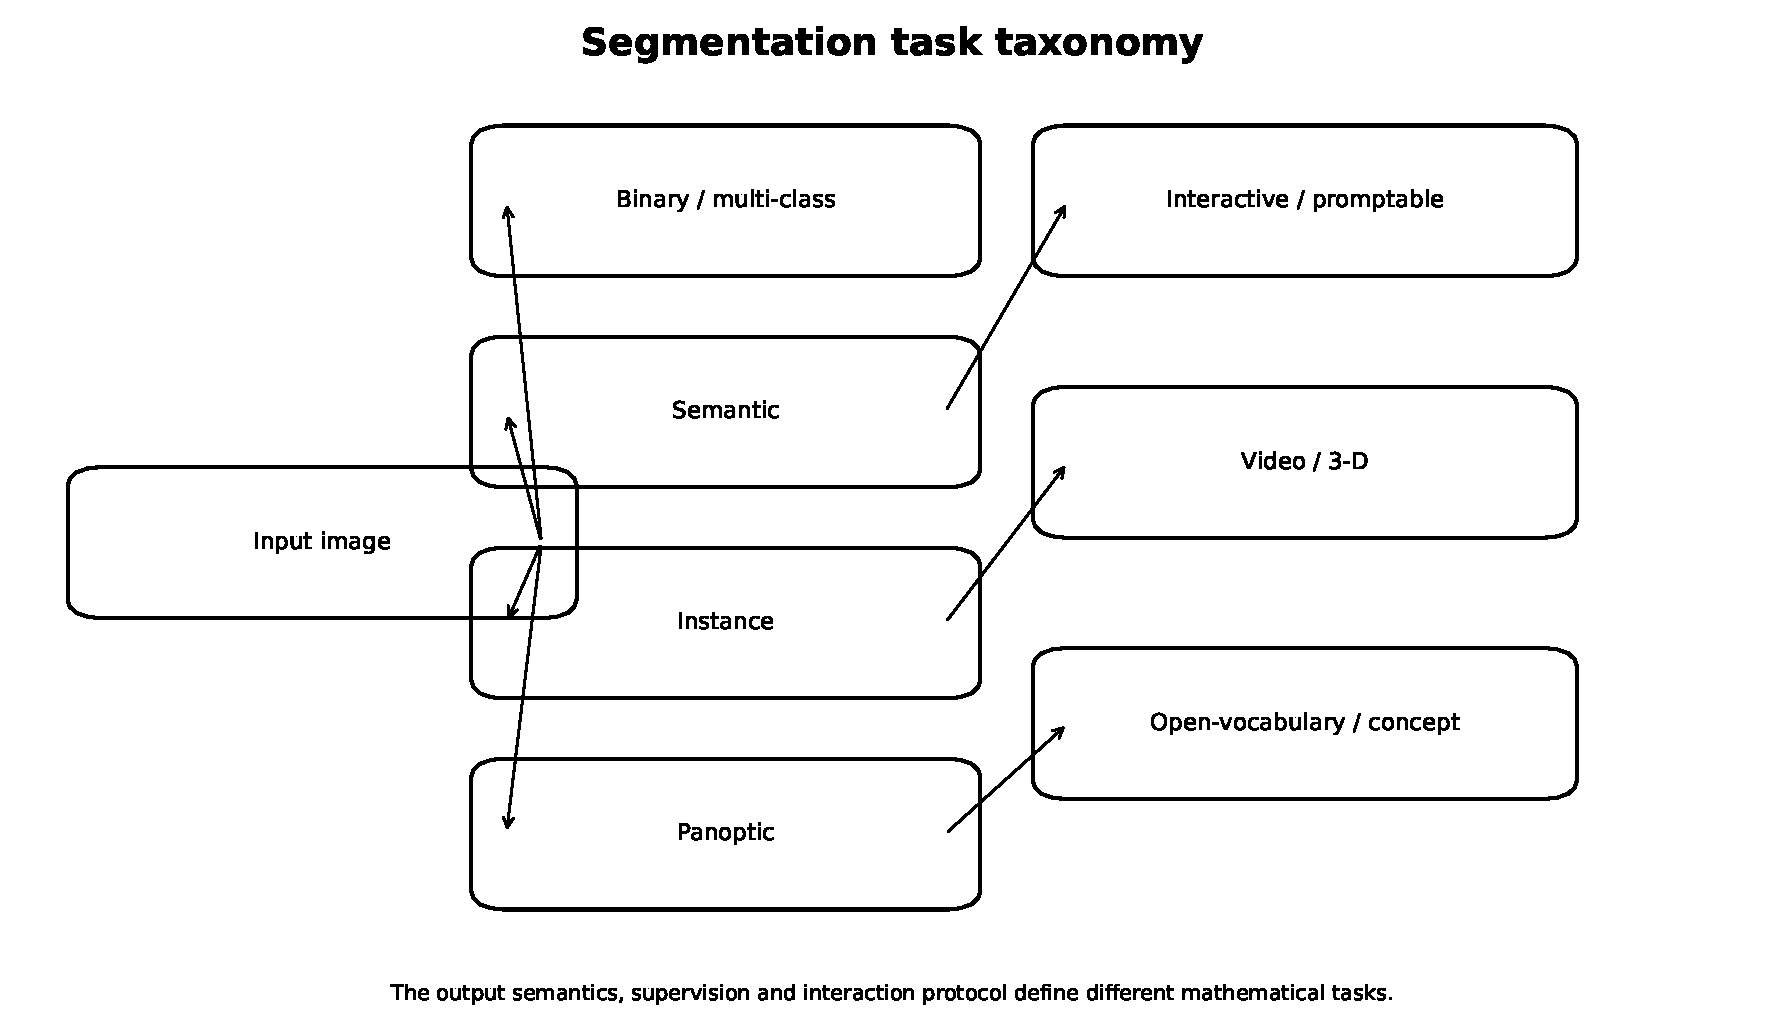
\includegraphics[width=0.93\textwidth]{fig01_segmentation_taxonomy.pdf}
\caption{رده‌بندی وظایف قطعه‌بندی بر اساس معنای خروجی، تعامل و بعد زمانی. یک معماری ممکن است چند وظیفه را پوشش دهد، اما قرارداد برچسب و معیار ارزیابی باید صریح باشد.}
\label{fig:seg-taxonomy}
\end{figure}

در ساده‌ترین حالت، هدف تقسیم \(\Omega\) به دو مجموعه پیش‌زمینه و پس‌زمینه است. در قطعه‌بندی چندکلاسه، هر پیکسل
یک رده می‌گیرد. در قطعه‌بندی معنایی، دو شیء هم‌رده یک برچسب مشترک دارند؛ در قطعه‌بندی نمونه‌ای، هویت هر نمونه نیز
جدا می‌شود؛ و در قطعه‌بندی پان‌اپتیک، همه پیکسل‌ها باید همزمان یک رده معنایی و در صورت شمارش‌پذیر بودن یک شناسه
نمونه دریافت کنند. قطعه‌بندی تعاملی خروجی را مشروط به click، box، scribble، mask یا متن می‌سازد. در ویدئو، ثبات
هویت و زمان نیز وارد مسئله می‌شود.

\begin{definition}[افراز]
خانواده \(\mathcal P=\{R_1,\ldots,R_K\}\) یک افراز از دامنه \(\Omega\) است اگر
\[
R_i\cap R_j=\varnothing\quad(i\neq j),\qquad
\bigcup_{k=1}^{K}R_k=\Omega.
\]
در instance segmentation معمولاً ماسک‌های پیش‌بینی‌شده می‌توانند پیش از حل تعارض هم‌پوشانی داشته باشند؛ در
panoptic segmentation خروجی نهایی باید افراز بدون هم‌پوشانی باشد.
\end{definition}

\subsection{قطعه‌بندی به عنوان تصمیم ساخت‌یافته}
برای زیان \(L(\widehat{\vect z},\vect z)\)، تصمیم بیزی به صورت
\[
\widehat{\vect z}_{\mathrm{Bayes}}
=\argmin_{\widehat{\vect z}}\E\!\left[L(\widehat{\vect z},\vect z)\mid\vect y\right]
\]
تعریف می‌شود. اگر زیان جمع پیکسلی و posterior مستقل باشد، تصمیم به \(HW\) طبقه‌بندی مستقل تجزیه می‌شود. اما
مرز، اتصال، اندازه، شکل و هویت نمونه‌ها مستقل نیستند؛ از این رو تقریب مستقل اغلب ماسک‌های دندانه‌دار، سوراخ‌دار یا
ناسازگار تولید می‌کند.

\begin{principlebox}
هر قطعه‌بندی سه لایه دارد: «چه چیزی را بخش‌بندی می‌کنیم؟»، «چه شواهدی از تصویر می‌گیریم؟» و «چه ساختاری را
مجاز می‌دانیم؟». خطای رایج این است که معماری را پیش از تعریف این سه لایه انتخاب کنیم.
\end{principlebox}

\section{قاعده بیز و پیدایش آستانه}
فرض کنید شدت \(Y\) از یکی از دو کلاس \(Z\in\{0,1\}\) آمده است. برای هزینه‌های
\(C_{ij}\) یعنی هزینه تصمیم \(i\) در حالی که کلاس واقعی \(j\) است، کلاس یک انتخاب می‌شود اگر
\[
(C_{10}-C_{00})P(Z=0\mid y)
< (C_{01}-C_{11})P(Z=1\mid y).
\]
با استفاده از بیز:
\[
\frac{p(y\mid Z=1)}{p(y\mid Z=0)}
>
\eta,
\qquad
\eta=
\frac{(C_{10}-C_{00})P(Z=0)}{(C_{01}-C_{11})P(Z=1)}.
\]
این رابطه یک آزمون نسبت درست‌نمایی است. بنابراین آستانه صرفاً یک ترفند هیستوگرام نیست؛ حالت خاص تصمیم بیزی است.

\subsection{دو کلاس گاوسی با واریانس برابر}
اگر
\[
Y\mid Z=k\sim\mathcal N(\mu_k,\sigma^2),
\]
آنگاه لگاریتم نسبت درست‌نمایی خطی است و آستانه به صورت
\[
t^*=\frac{\mu_0+\mu_1}{2}
+\frac{\sigma^2}{\mu_1-\mu_0}\log\eta
\]
به دست می‌آید. برای prior و هزینه برابر، \(t^*=(\mu_0+\mu_1)/2\). اگر واریانس‌ها متفاوت باشند، معادله تصمیم
درجه دوم است و حتی ممکن است ناحیه تصمیم یک بازه محدود باشد، نه یک نیم‌خط.

\begin{warningbox}
وجود دو قله در هیستوگرام شرط لازم یا کافی برای قطعه‌بندی خوب نیست. دو ناحیه می‌توانند شدت مشابه و بافت متفاوت
داشته باشند، یا یک شیء به علت سایه و روشنایی چند قله تولید کند. هیستوگرام مکان پیکسل را حذف می‌کند.
\end{warningbox}

\section{آستانه‌گذاری سراسری}
\subsection{فرمول‌بندی عمومی}
برای تصویر خاکستری نرمال‌شده \(y_p\in[0,1]\)، قطعه‌بندی دودویی با آستانه \(t\) برابر است با
\[
m_p(t)=\ind[y_p>t].
\]
هزینه انتخاب \(t\) می‌تواند بر جدایی آماری، entropy، خطای مدل مخلوط یا معیار پایین‌دست بنا شود. اگر آستانه پس از
دیدن ground truth انتخاب شود، نتیجه خوش‌بینانه و غیرقابل تعمیم است؛ بنابراین پارامتر باید روی validation یا با معیار
بدون نظارت انتخاب شود.

\subsection{روش Otsu: استخراج دقیق}
فرض کنید هیستوگرام نرمال‌شده \(p_i=n_i/N\) برای سطوح \(i=0,\ldots,L-1\) باشد. برای آستانه \(t\):
\[
\omega_0(t)=\sum_{i=0}^{t}p_i,
\qquad
\omega_1(t)=1-\omega_0(t),
\]
\[
\mu_0(t)=\frac{1}{\omega_0(t)}\sum_{i=0}^{t}i p_i,
\qquad
\mu_1(t)=\frac{1}{\omega_1(t)}\sum_{i=t+1}^{L-1}i p_i.
\]
واریانس درون‌کلاسی و بین‌کلاسی عبارت‌اند از
\[
\sigma_w^2(t)=\omega_0\sigma_0^2+\omega_1\sigma_1^2,
\qquad
\sigma_b^2(t)=\omega_0\omega_1(\mu_0-\mu_1)^2.
\]
از تجزیه واریانس کل داریم
\[
\sigma_T^2=\sigma_w^2(t)+\sigma_b^2(t),
\]
که مستقل از \(t\) است؛ پس کمینه‌کردن واریانس درون‌کلاسی معادل بیشینه‌کردن واریانس بین‌کلاسی است:
\[
t_{\mathrm{Otsu}}=\argmax_t \sigma_b^2(t).
\]
با تعریف میانگین تجمعی \(\mu(t)=\sum_{i=0}^{t}i p_i\) و میانگین کل \(\mu_T\)، فرم پایدارتر محاسباتی
\[
\sigma_b^2(t)=
\frac{\left(\mu_T\omega_0(t)-\mu(t)\right)^2}
{\omega_0(t)(1-\omega_0(t))}
\]
به دست می‌آید. آستانه‌هایی که یکی از کلاس‌ها وزن صفر دارد حذف می‌شوند.

\begin{theorembox}{پیچیدگی Otsu}
ساخت هیستوگرام \(O(N)\) و پیمایش آستانه‌ها \(O(L)\) است. با مجموع‌های تجمعی، برای هر \(t\) محاسبه ثابت انجام
می‌شود؛ بنابراین کل پیچیدگی \(O(N+L)\) و حافظه \(O(L)\) است.
\end{theorembox}

\begin{figure}[H]
\centering
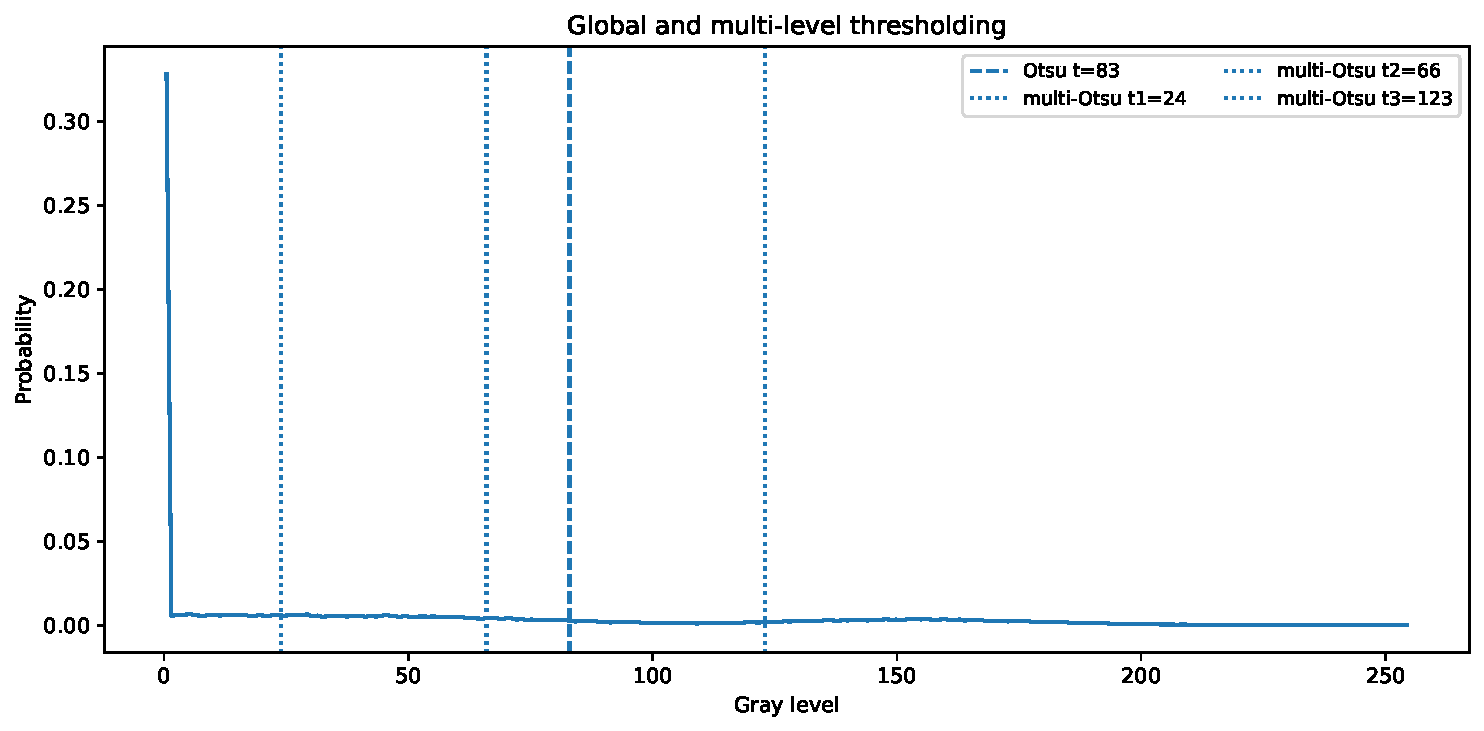
\includegraphics[width=0.84\textwidth]{fig02_otsu_histogram.pdf}
\caption{آستانه Otsu و چندآستانه‌ای روی یک تصویر مصنوعی. انتخاب صرفاً از هیستوگرام انجام می‌شود و مکان پیکسل‌ها در معیار حضور ندارد.}
\label{fig:otsu}
\end{figure}

\begin{algorithmbox}{الگوریتم ۱: Otsu پایدار با مجموع تجمعی}
\begin{enumerate}
\item هیستوگرام \(h_i\) را بسازید و \(p_i=h_i/N\) را محاسبه کنید.
\item آرایه‌های تجمعی \(\omega(t)=\sum_{i\leq t}p_i\) و \(\mu(t)=\sum_{i\leq t}i p_i\) را بسازید.
\item برای هر \(t\) با \(0<\omega(t)<1\)، مقدار \(\sigma_b^2(t)\) را محاسبه کنید.
\item اگر چند آستانه بیشینه برابر دارند، قرارداد tie-breaking را ثبت کنید؛ انتخاب میانگین بازه بیشینه معمولاً پایدارتر است.
\item آستانه را به مقیاس شدت اصلی بازگردانید و ماسک را با قرارداد \(>\) یا \(\geq\) بسازید.
\end{enumerate}
\textbf{آزمون صحت:} روی تصویر ثابت، هیستوگرام تک‌جرمی و تصویر دو سطحی رفتار مورد انتظار را بررسی کنید.
\end{algorithmbox}

\subsection{تفسیر Otsu به عنوان خوشه‌بندی یک‌بعدی}
Otsu برای دو کلاس معادل انتخاب برشی است که مجموع خطای مربعی درون دو خوشه شدت را کمینه می‌کند. در نتیجه، با
k-means یک‌بعدی ارتباط مستقیم دارد، اما قید می‌کند خوشه‌ها در محور شدت پیوسته و با یک آستانه جدا شوند. این قید
سرعت و تفسیرپذیری می‌دهد، ولی برای چگالی‌های درهم‌رفته یا چندوجهی محدودکننده است.

\subsection{چندآستانه‌ای و برنامه‌ریزی پویا}
برای \(K\) کلاس و آستانه‌های \(t_1<\cdots<t_{K-1}\)، هدف کمینه‌سازی
\[
J(t_1,\ldots,t_{K-1})=
\sum_{k=1}^{K}\sum_{i\in I_k}p_i(i-\mu_k)^2
\]
است. جست‌وجوی مستقیم \(O(L^{K-1})\) است. اگر هزینه یک بازه \([a,b]\) را
\[
C(a,b)=\sum_{i=a}^{b}p_i(i-\mu_{a:b})^2
\]
بنامیم، برنامه‌ریزی پویا می‌نویسد
\[
D(k,b)=\min_{a< b}\{D(k-1,a)+C(a+1,b)\}.
\]
با پیش‌محاسبه جمع‌های \(p_i\)، \(ip_i\) و \(i^2p_i\)، هزینه هر بازه در زمان ثابت محاسبه می‌شود و پیچیدگی
معمول \(O(KL^2)\) است. backtracking آستانه‌ها را بازیابی می‌کند.

\begin{algorithmbox}{الگوریتم ۲: Multi-Otsu با برنامه‌ریزی پویا}
\begin{enumerate}
\item سه مجموع تجمعی \(S_0,S_1,S_2\) را برای \(p_i,ip_i,i^2p_i\) بسازید.
\item با آنها \(C(a,b)=S_2-S_1^2/S_0\) را برای بازه‌های معتبر محاسبه کنید.
\item جدول \(D(k,b)\) و جدول والد \(P(k,b)\) را پر کنید.
\item از \(D(K,L-1)\) به عقب حرکت کنید تا \(K-1\) آستانه به دست آید.
\item کلاس‌های بسیار کوچک را با حداقل جرم یا جریمه تعداد کلاس کنترل کنید.
\end{enumerate}
\end{algorithmbox}

\subsection{آستانه entropy و minimum error}
در روش maximum entropy، برای هر سوی آستانه entropy شرطی محاسبه می‌شود:
\[
H_0(t)=-\sum_{i\le t}\frac{p_i}{\omega_0}\log\frac{p_i}{\omega_0},
\qquad
H_1(t)=-\sum_{i>t}\frac{p_i}{\omega_1}\log\frac{p_i}{\omega_1},
\]
و \(H_0+H_1\) بیشینه می‌شود. روش Kittler--Illingworth هیستوگرام را مخلوط دو گاوسی فرض و خطای طبقه‌بندی
برآوردشده را کمینه می‌کند. این روش هنگامی مناسب‌تر است که مدل شدت واقعاً نزدیک مخلوط پارامتری باشد، ولی در برابر
برآورد ناپایدار واریانس کلاس کوچک حساس است.

\subsection{روش‌های ساده اما مفید}
\begin{itemize}
\item \textbf{Percentile:} وقتی نسبت تقریبی پیش‌زمینه معلوم است؛ برای کنترل کیفیت خط تولید مفید است.
\item \textbf{Triangle:} برای هیستوگرام یک‌قله‌ای با دنباله بلند؛ فاصله نقاط هیستوگرام از خط قله تا انتهای دنباله را بیشینه می‌کند.
\item \textbf{Hysteresis:} دو آستانه \(t_l<t_h\)؛ پیکسل قوی seed است و پیکسل ضعیف فقط در صورت اتصال پذیرفته می‌شود.
\item \textbf{Threshold روی نسبت یا شاخص:} در تصاویر چندطیفی، متغیری مانند \((a-b)/(a+b)\) گاه جدایی فیزیکی بهتری از شدت خام می‌دهد.
\end{itemize}

\section{آستانه‌گذاری محلی و روشنایی ناهمگن}
مدل ساده سند یا صحنه سایه‌دار را می‌توان چنین نوشت:
\[
y(p)=\ell(p)r(p)+n(p),
\]
که \(\ell\) روشنایی آهسته‌تغییر و \(r\) بازتاب است. آستانه جهانی تغییرات \(\ell\) را با تغییر کلاس اشتباه می‌گیرد.
راه‌حل‌ها یا \(\ell\) را برآورد و حذف می‌کنند، یا آستانه را تابع مکان می‌سازند: \(t=t(p)\).

\subsection{میانگین محلی و تصویر انتگرالی}
برای پنجره \(W_p\):
\[
\mu_p=\frac{1}{|W_p|}\sum_{q\in W_p}y_q,
\qquad
m_p=\ind[y_p>\mu_p-c].
\]
تصویر انتگرالی
\[
I(r,c)=\sum_{i\le r}\sum_{j\le c}y(i,j)
\]
جمع هر مستطیل را با چهار دسترسی محاسبه می‌کند؛ بنابراین میانگین محلی برای همه پیکسل‌ها در \(O(N)\) مستقل از
اندازه پنجره قابل محاسبه است.

\subsection{Niblack و Sauvola}
Niblack از
\[
t_p=\mu_p+k\sigma_p
\]
استفاده می‌کند. در سند، علامت و مقدار \(k\) به قرارداد foreground بستگی دارد. Sauvola برای جلوگیری از تولید نویز
در نواحی کم‌واریانس پیشنهاد می‌کند
\[
t_p=\mu_p\left[1+k\left(\frac{\sigma_p}{R}-1\right)\right],
\]
که \(R\) دامنه مرجع انحراف معیار است. وقتی \(\sigma_p\ll R\)، آستانه از میانگین فاصله می‌گیرد و حساسیت به
پس‌زمینه هموار کاهش می‌یابد.

\begin{figure}[H]
\centering
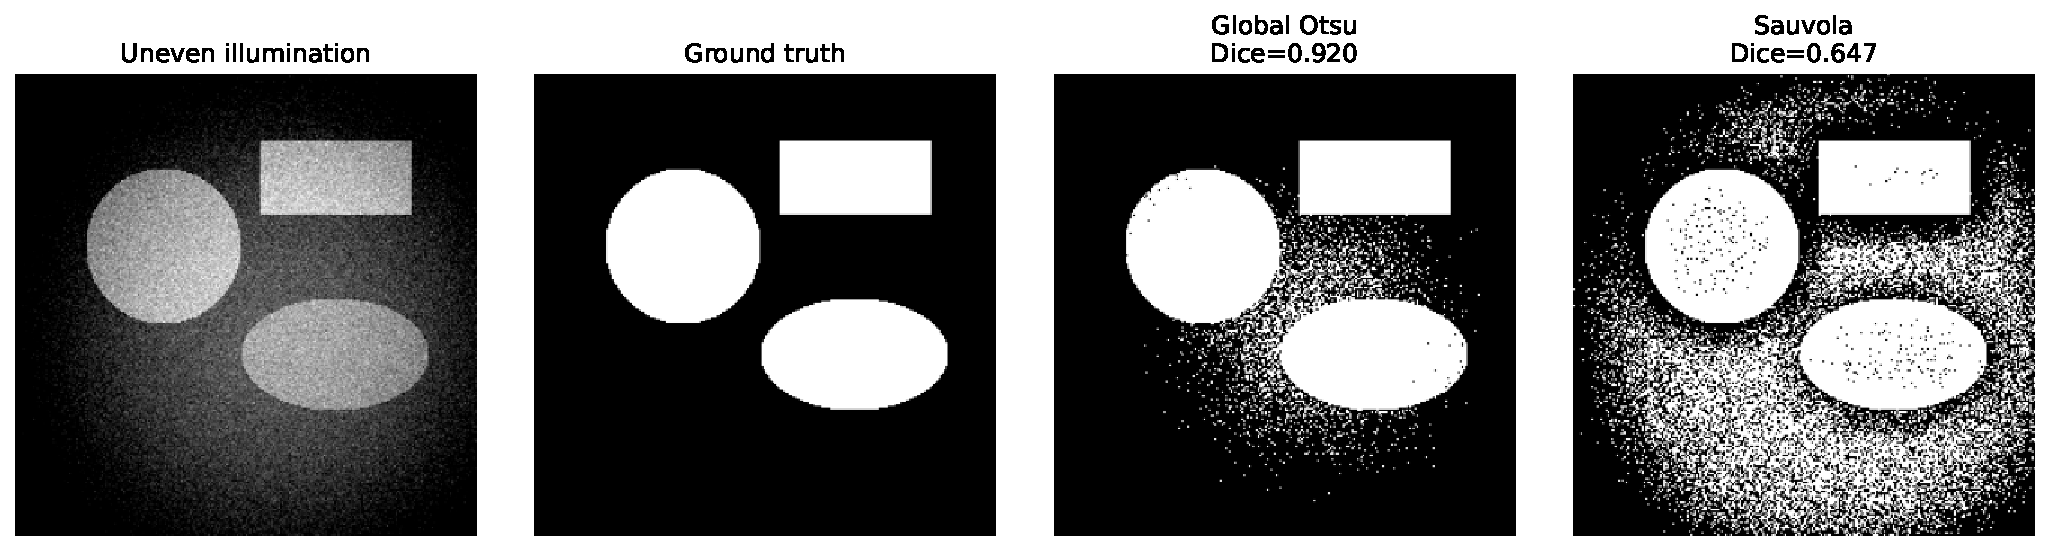
\includegraphics[width=0.98\textwidth]{fig03_adaptive_thresholding.pdf}
\caption{نمونه شکست آستانه جهانی زیر روشنایی ناهمگن و نقش آستانه محلی. کیفیت به اندازه پنجره و نسبت مقیاس روشنایی به شیء وابسته است؛ یک روش محلی الزاماً در هر تصویر بهتر نیست.}
\label{fig:adaptive-threshold}
\end{figure}

\begin{algorithmbox}{الگوریتم ۳: آستانه محلی با تصویر انتگرالی}
\begin{enumerate}
\item تصویر و مربع آن را به float تبدیل کنید و دو تصویر انتگرالی \(I\) و \(I_2\) بسازید.
\item برای هر پیکسل، مرز پنجره را با قرارداد مشخص clip یا reflect کنید.
\item جمع و جمع مربع را با چهار گوشه بازیابی و \(\mu_p,\sigma_p\) را محاسبه کنید.
\item آستانه Niblack، Sauvola یا فرمول سفارشی را اعمال کنید.
\item اجزای کوچک و حفره‌ها را تنها در صورت وجود دلیل هندسی اصلاح کنید؛ post-processing بخشی از مدل است و باید گزارش شود.
\end{enumerate}
\textbf{پیچیدگی:} زمان \(O(N)\)، حافظه \(O(N)\). برای تصاویر عظیم می‌توان پردازش tiled با halo انجام داد.
\end{algorithmbox}

\begin{warningbox}
پنجره بسیار کوچک نویز را دنبال می‌کند؛ پنجره بسیار بزرگ دوباره به آستانه جهانی نزدیک می‌شود. اندازه پنجره باید از
مقیاس stroke یا شیء و مقیاس تغییر روشنایی استخراج شود، نه با آزمون روی test set.
\end{warningbox}

\subsection{آستانه دوبعدی و ویژگی‌های چندکاناله}
هیستوگرام مشترک شدت و میانگین محلی، شدت و گرادیان، یا دو کانال رنگ می‌تواند ابهام یک‌بعدی را کاهش دهد. اما تعداد
binها با بعد به صورت نمایی رشد می‌کند. در ابعاد بالاتر، تخمین چگالی، GMM یا classifier معمولاً مناسب‌تر از هیستوگرام
چندبعدی خام است.

\begin{workshopbox}[آستانه‌گذاری قابل ممیزی]
برای یک مجموعه شامل سند، سلول، قطعه صنعتی و تصویر سایه‌دار، Otsu، Triangle، Sauvola و یک آستانه بیزی را مقایسه
کنید. علاوه بر Dice، حساسیت به gamma، blur، نویز و resize را گزارش کنید. نمودار آستانه منتخب در هر perturbation
بهتر از یک جدول تک‌عددی رفتار روش را آشکار می‌کند.
\end{workshopbox}

\section{رشد ناحیه و اتصال}
آستانه‌گذاری می‌پرسد «مقدار این پیکسل چیست؟»؛ رشد ناحیه می‌پرسد «آیا این پیکسل به یک ناحیه موجود و سازگار متصل
است؟». از seedهای \(S_k\) شروع می‌کنیم و پیکسل مرزی \(q\) را به ناحیه \(R_k\) می‌افزاییم اگر
\[
q\in\mathcal N(R_k),
\qquad
P(q,R_k)=\mathrm{true}.
\]
یک predicate ساده
\[
P(q,R_k)=\ind\left[\abs{y_q-\mu(R_k)}\le\tau\right]
\]
است. چون \(\mu(R_k)\) با رشد تغییر می‌کند، ترتیب پردازش ممکن است نتیجه را تغییر دهد. استفاده از صف اولویت بر
اساس هزینه الحاق این وابستگی را کنترل می‌کند.

\begin{figure}[H]
\centering
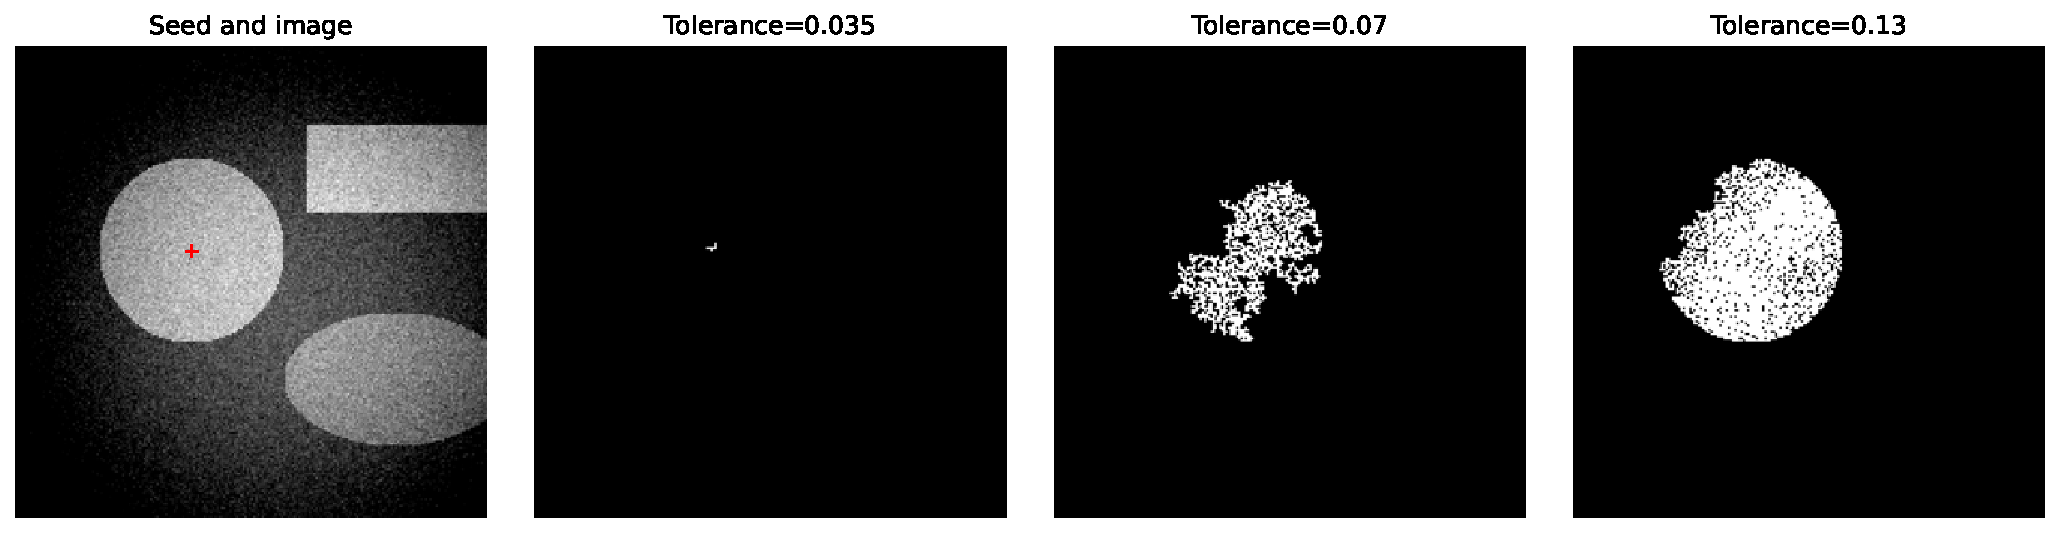
\includegraphics[width=0.96\textwidth]{fig04_region_growing.pdf}
\caption{حساسیت رشد ناحیه به آستانه سازگاری. مقدار کوچک کم‌قطعه‌بندی و مقدار بزرگ leakage ایجاد می‌کند؛ seed و مدل ناحیه بخشی از مسئله‌اند.}
\label{fig:region-growing}
\end{figure}

\begin{algorithmbox}{الگوریتم ۴: رشد ناحیه صف‌محور}
\begin{enumerate}
\item seedها را اعتبارسنجی و برچسب اولیه را ایجاد کنید.
\item همسایه‌های seed را در صف یا priority queue وارد کنید.
\item کم‌هزینه‌ترین پیکسل \(q\) را خارج و هزینه آن نسبت به ناحیه‌های مجاور را محاسبه کنید.
\item اگر بهترین هزینه کمتر از \(\tau\) است، برچسب را تثبیت و آمار ناحیه را آنلاین به‌روزرسانی کنید.
\item همسایه‌های برچسب‌نخورده را وارد صف کنید؛ در تعارض، قاعده tie-breaking را ثبت کنید.
\item در پایان، شرط اندازه، compactness یا اتصال را بررسی کنید.
\end{enumerate}
\textbf{پیچیدگی:} با صف ساده \(O(N)\) و با heap معمولاً \(O(N\log N)\). هر پیکسل باید تعداد محدودی وارد صف شود.
\end{algorithmbox}

\subsection{انتخاب seed}
seed می‌تواند دستی، از آستانه قوی، extrema تبدیل فاصله، marker مورفولوژیک، detection، نقطه کاربر یا خروجی شبکه
باشد. کیفیت seed در روش‌های تعاملی باید با «تعداد تعامل تا رسیدن به کیفیت هدف» سنجیده شود، نه فقط کیفیت پس از
تعداد نامحدود click.

\subsection{Split and merge}
دامنه ابتدا به بلوک‌هایی تقسیم می‌شود. اگر predicate همگنی برقرار نباشد، بلوک به چهار فرزند شکسته می‌شود؛ سپس
بلوک‌های مجاور سازگار ادغام می‌شوند. ساختار quadtree محاسبه را منظم می‌کند، ولی مرزهای بلوکی مصنوعی و وابستگی
به alignment ایجاد می‌کند. ادغام پس از split برای حذف این اثر ضروری است.

\subsection{رابطه با watershed}
watershed نشان‌محور را می‌توان رشد همزمان چند ناحیه روی توپوگرافی گرادیان دید. تفاوت اصلی آن است که اولویت رشد
از ارتفاع یا هزینه مسیر می‌آید و خط جدایی در برخورد جبهه‌ها ساخته می‌شود. ابزارهای فصل هفتم برای marker، بازسازی
مورفولوژیک و کنترل minima مستقیماً در اینجا استفاده می‌شوند.

\section{خوشه‌بندی و مدل‌های مخلوط}
\subsection{k-means در فضای ویژگی}
برای ویژگی \(\vect x_p\in\R^d\) شامل رنگ، شدت، بافت و مختصات، k-means حل می‌کند
\[
\min_{\{z_p\},\{\vect\mu_k\}}
\sum_{p\in\Omega}\norm{\vect x_p-\vect\mu_{z_p}}_2^2.
\]
الگوریتم Lloyd دو گام دارد:
\[
z_p\leftarrow\argmin_k\norm{\vect x_p-\vect\mu_k}^2,
\qquad
\vect\mu_k\leftarrow\frac{1}{|R_k|}\sum_{p:z_p=k}\vect x_p.
\]
هر گام تابع هدف را کاهش می‌دهد، اما تضمین تنها همگرایی به مینیمم محلی است. k-means++، چند restart و ثبت بهترین
تابع هدف ضروری‌اند.

\begin{keybox}[مقیاس ویژگی]
اگر \(\vect x_p=[L,a,b,\alpha x,\alpha y]\) باشد، پارامتر \(\alpha\) نسبت شباهت ظاهری به فشردگی مکانی را
تعیین می‌کند. بدون استانداردسازی، کانالی با دامنه بزرگ هندسه فاصله را تسخیر می‌کند. انتخاب فضای \lr{Lab} یا ویژگی
آموخته‌شده نیز بخشی از فرض مدل است.
\end{keybox}

\subsection{GMM و الگوریتم EM}
در مدل مخلوط گاوسی
\[
p(\vect x)=\sum_{k=1}^{K}\pi_k\mathcal N(\vect x;\vect\mu_k,\mat\Sigma_k),
\qquad \sum_k\pi_k=1.
\]
متغیر پنهان \(z_p\) عضویت کلاس است. در گام E مسئولیت‌ها
\[
\gamma_{pk}=P(z_p=k\mid\vect x_p)
=\frac{\pi_k\mathcal N(\vect x_p;\vect\mu_k,\mat\Sigma_k)}
{\sum_j\pi_j\mathcal N(\vect x_p;\vect\mu_j,\mat\Sigma_j)}
\]
و در گام M
\[
N_k=\sum_p\gamma_{pk},\quad
\pi_k=\frac{N_k}{N},\quad
\vect\mu_k=\frac{1}{N_k}\sum_p\gamma_{pk}\vect x_p,
\]
\[
\mat\Sigma_k=\frac{1}{N_k}\sum_p\gamma_{pk}
(\vect x_p-\vect\mu_k)(\vect x_p-\vect\mu_k)\trans
\]
به‌روزرسانی می‌شوند. EM درست‌نمایی را کاهش نمی‌دهد، اما به مقداردهی اولیه و فروپاشی کوواریانس حساس است؛ افزودن
\(\epsilon\mat I\) و حداقل جرم مؤلفه لازم است.

\begin{figure}[H]
\centering
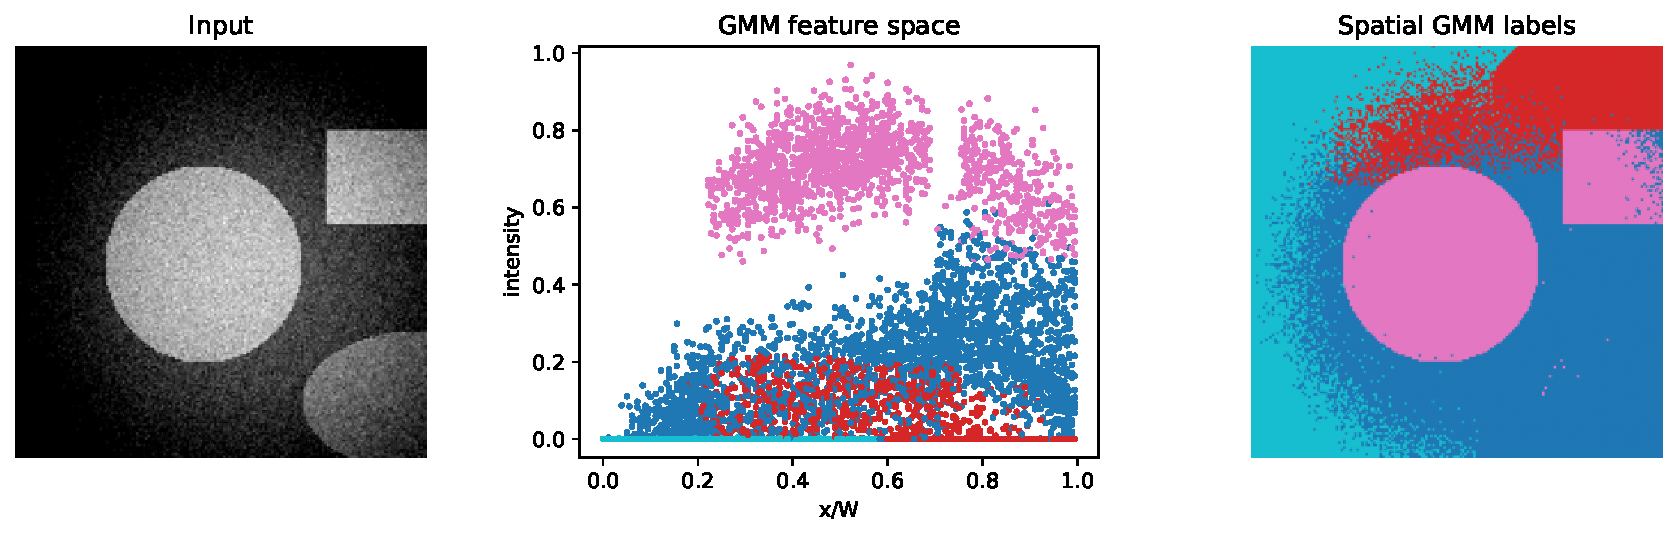
\includegraphics[width=0.94\textwidth]{fig05_gmm_clustering.pdf}
\caption{خوشه‌بندی GMM در فضایی که شدت و مختصات را ترکیب می‌کند. افزودن مکان اتصال را تضمین نمی‌کند، اما از پخش‌شدن یک کلاس ظاهری در سراسر تصویر می‌کاهد.}
\label{fig:gmm}
\end{figure}

\begin{algorithmbox}{الگوریتم ۵: EM پایدار برای قطعه‌بندی GMM}
\begin{enumerate}
\item ویژگی‌ها را با آمار train یا همان تصویر، طبق پروتکل ثابت، نرمال کنید.
\item پارامترها را با k-means++ یا چند مقداردهی اولیه بسازید.
\item در E-step، احتمال‌ها را در فضای log و با log-sum-exp محاسبه کنید.
\item در M-step، وزن، میانگین و کوواریانس را به‌روزرسانی و regularization قطری اضافه کنید.
\item معیار توقف را بر تغییر log-likelihood نسبی و حداکثر iteration تعریف کنید.
\item برچسب نهایی را با \(\argmax\gamma_{pk}\) و عدم‌قطعیت را با entropy مسئولیت‌ها گزارش کنید.
\end{enumerate}
\textbf{پیچیدگی:} برای کوواریانس کامل تقریباً \(O(TNKd^2)\)؛ کوواریانس قطری هزینه را به \(O(TNKd)\) کاهش می‌دهد.
\end{algorithmbox}

\subsection{Fuzzy c-means}
برای عضویت نرم \(u_{pk}\in[0,1]\) و \(\sum_k u_{pk}=1\):
\[
J_m=\sum_p\sum_k u_{pk}^{m}\norm{\vect x_p-\vect\mu_k}^2,
\qquad m>1.
\]
پارامتر \(m\) میزان fuzziness را کنترل می‌کند. عضویت نرم برای partial volume در MRI یا مرزهای مخلوط مفید است،
اما membership لزوماً احتمال کالیبره نیست.

\subsection{Mean shift}
Mean shift مد چگالی KDE را دنبال می‌کند. برای kernel \(K_h\)، بردار mean-shift اختلاف میانگین وزن‌دار همسایگی و
نقطه جاری است. مزیت آن نیازنداشتن به تعداد خوشه از پیش است؛ عیب آن حساسیت شدید به bandwidth و هزینه بالا در
ابعاد و داده بزرگ است.

\subsection{افزودن ساختار مکانی}
یک راه ساده افزودن مختصات به ویژگی است؛ راه اصولی‌تر افزودن prior روی برچسب‌هاست:
\[
p(\vect z)\propto\exp\left(-\beta\sum_{(p,q)\in\mathcal E}\ind[z_p\neq z_q]\right).
\]
این مدل Potts مرز را جریمه می‌کند. posterior دیگر به پیکسل‌ها تجزیه نمی‌شود و به روش‌های گرافی، belief propagation،
mean-field یا روش واریاسیونی نیاز دارد.

\section{قطعه‌بندی واریاسیونی: از Mumford--Shah تا Chan--Vese}
\subsection{تابع Mumford--Shah}
برای تصویر \(y:\Omega\to\R\)، تابع piecewise-smooth \(u\) و مجموعه ناپیوستگی \(C\):
\[
E(u,C)=\int_{\Omega\setminus C}(u-y)^2\,d\vect x
+\alpha\int_{\Omega\setminus C}\norm{\nabla u}^2\,d\vect x
+\beta\,\mathcal H^1(C).
\]
ترم نخست fidelity، ترم دوم همواری درون ناحیه و ترم سوم طول مرز است. بهینه‌سازی مستقیم روی تابع و مجموعه منحنی
دشوار است. تقریب Ambrosio--Tortorelli یا مدل‌های piecewise constant این مانع را کاهش می‌دهند.

\subsection{مدل قطعه‌ای ثابت و انرژی Chan--Vese}
برای ناحیه داخل منحنی \(C\) و خارج آن، شدت با ثابت‌های \(c_1,c_2\) تقریب زده می‌شود:
\begin{align}
E(C,c_1,c_2)={}&\mu\,\mathrm{Length}(C)
+\nu\,\mathrm{Area}(\mathrm{inside}(C))\\
&+\lambda_1\int_{\mathrm{inside}(C)}(y-c_1)^2\,d\vect{x}
+\lambda_2\int_{\mathrm{outside}(C)}(y-c_2)^2\,d\vect{x}.
\end{align}
برای منحنی ثابت، کمینه نسبت به \(c_1,c_2\) میانگین نواحی است. منحنی را با level-set
\(C=\{\vect x:\phi(\vect x)=0\}\) نمایش می‌دهیم. با تابع Heaviside \(H(\phi)\) و دلتا \(\delta(\phi)\):
\begin{align}
E(\phi)={}&\mu\int\delta(\phi)\norm{\nabla\phi}\,d\vect{x}
+\nu\int H(\phi)\,d\vect{x}\\
&+\lambda_1\int(y-c_1)^2H(\phi)\,d\vect{x}
+\lambda_2\int(y-c_2)^2(1-H(\phi))\,d\vect{x}.
\end{align}
نزول گرادیان شکل تقریبی
\[
\frac{\partial\phi}{\partial t}=\delta_\epsilon(\phi)
\left[
\mu\,\mathrm{div}\left(\frac{\nabla\phi}{\norm{\nabla\phi}}\right)
-\nu-\lambda_1(y-c_1)^2+\lambda_2(y-c_2)^2
\right]
\]
دارد. curvature مرز را هموار و اختلاف خطاهای ناحیه‌ای جبهه را هدایت می‌کند.

\begin{figure}[H]
\centering
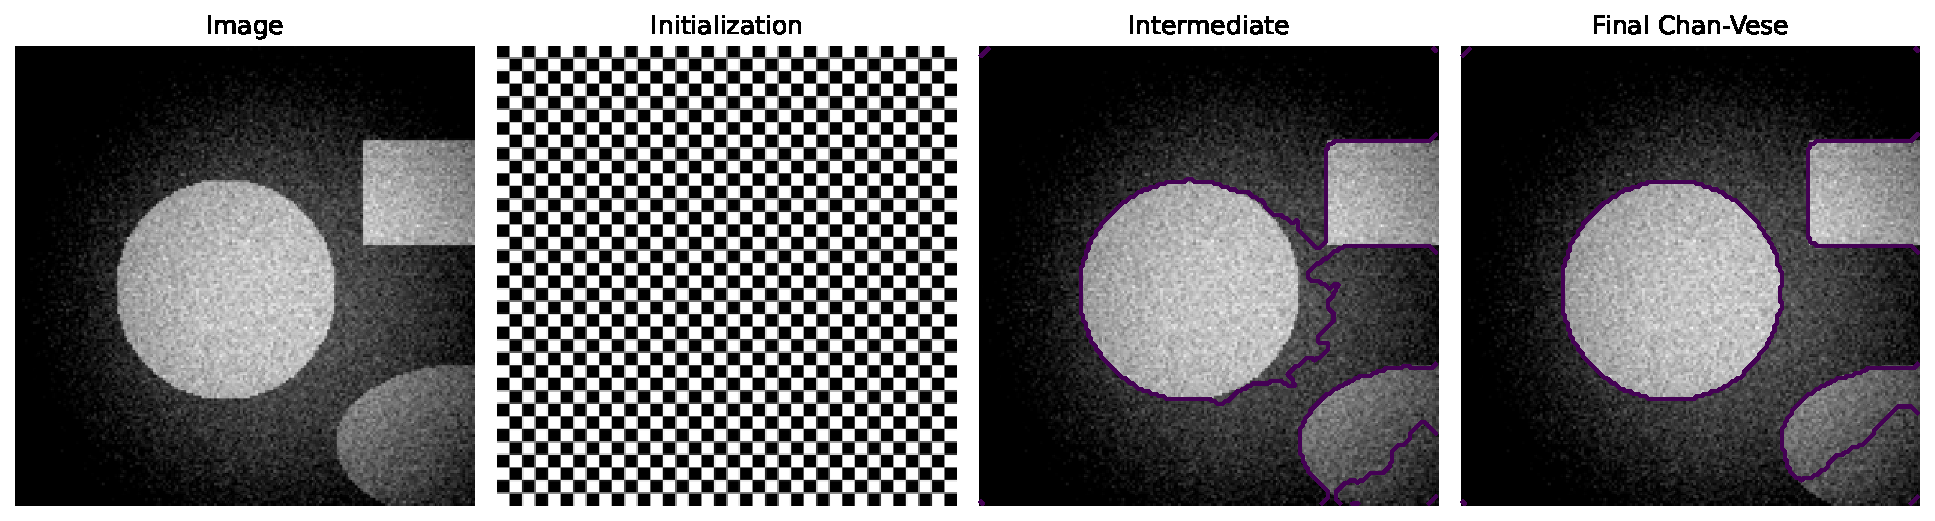
\includegraphics[width=0.95\textwidth]{fig08_chan_vese.pdf}
\caption{تکامل یک contour ناحیه‌محور. مدل Chan--Vese برای مرزهایی که گرادیان ضعیف دارند مفید است، ولی فرض ثابت‌بودن شدت هر ناحیه در روشنایی ناهمگن می‌شکند.}
\label{fig:chan-vese}
\end{figure}

\begin{proofbox}[چرا میانگین ناحیه به دست می‌آید؟]
برای ناحیه ثابت \(R\)، تابع \(F(c)=\int_R(y-c)^2d\vect x\) را مشتق می‌گیریم:
\[
F'(c)=2\int_R(c-y)d\vect x=0
\quad\Rightarrow\quad
c=\frac{1}{|R|}\int_R y\,d\vect x.
\]
پس Chan--Vese در هر iteration یک مدل دو-میانگینی می‌سازد و مرز را با regularization هندسی به آن سازگار می‌کند.
\end{proofbox}

\subsection{Geodesic active contour}
مدل edge-based از تابع توقف
\[
g(\abs{\nabla G_\sigma*y})=\frac{1}{1+\abs{\nabla G_\sigma*y}^2}
\]
استفاده می‌کند و انرژی طول وزن‌دار \(\int_C g\,ds\) را کمینه می‌سازد. گرادیان قوی \(g\) را کوچک و contour را
متوقف می‌کند. در مرز ضعیف، gap یا بافت، leakage رخ می‌دهد؛ در مقابل Chan--Vese از آمار ناحیه استفاده می‌کند.

\subsection{مدل‌های محلی و چندفازی}
برای روشنایی ناهمگن، \(c_1,c_2\) را تابع مکان یا میانگین kernel-weighted می‌سازند. مدل‌های multiphase با چند level-set
تا \(2^m\) ناحیه تولید می‌کنند. افزایش انعطاف، هزینه بهینه‌سازی و خطر مینیمم محلی را نیز افزایش می‌دهد.

\begin{algorithmbox}{الگوریتم ۶: Chan--Vese با level set}
\begin{enumerate}
\item \(\phi^0\) را از دایره، checkerboard یا seed بسازید؛ فاصله علامت‌دار شروع مناسبی است.
\item \(H_\epsilon,\delta_\epsilon\) را با تقریب نرم تعریف کنید.
\item \(c_1,c_2\) را از میانگین‌های وزن‌دار \(H_\epsilon(\phi)\) محاسبه کنید.
\item curvature و نیروی داده را محاسبه و \(\phi\) را با گام پایدار به‌روزرسانی کنید.
\item در صورت روش کلاسیک، هر چند iteration reinitialization انجام دهید؛ یا از level-set فاصله‌منظم استفاده کنید.
\item توقف را بر تغییر انرژی، تغییر ماسک و سقف iteration مشترک تعریف کنید.
\end{enumerate}
\end{algorithmbox}

\section{مدل‌های گرافی و انرژی گسسته}
\subsection{MRF/CRF و انرژی Potts}
یک انرژی رایج چندکلاسه:
\[
E(\vect z)=\sum_p D_p(z_p)+\lambda\sum_{(p,q)\in\mathcal E}w_{pq}\ind[z_p\neq z_q].
\]
ترم unary از مدل شدت، شبکه یا prompt می‌آید. وزن
\[
w_{pq}=\exp\left(-\beta\norm{\vect y_p-\vect y_q}^2\right)\frac{1}{\dist(p,q)}
\]
جریمه قطع را در مرز ظاهری کاهش می‌دهد. این انرژی posterior منفی-log یک MRF یا CRF زوجی است.

\subsection{برش s--t برای مسئله دودویی}
برای \(z_p\in\{0,1\}\)، گرافی با source، sink، پیکسل‌ها، t-linkهای unary و n-linkهای pairwise ساخته می‌شود. هر
برش source--sink یک برچسب‌گذاری دودویی و ظرفیت برش برابر انرژی آن است. قضیه max-flow/min-cut تضمین می‌کند
کمینه سراسری با max-flow به دست آید، اگر ترم زوجی زیرمدولار باشد.

\begin{theorem}[شرط زیرمدولار زوج دودویی]
برای هزینه \(V(z_p,z_q)\)، نمایش دقیق با برش گراف زمانی ممکن است که
\[
V(0,0)+V(1,1)\le V(0,1)+V(1,0).
\]
این شرط یعنی ترجیح برچسب یکسان از نظر انرژی ناسازگار نیست.
\end{theorem}

\begin{figure}[H]
\centering
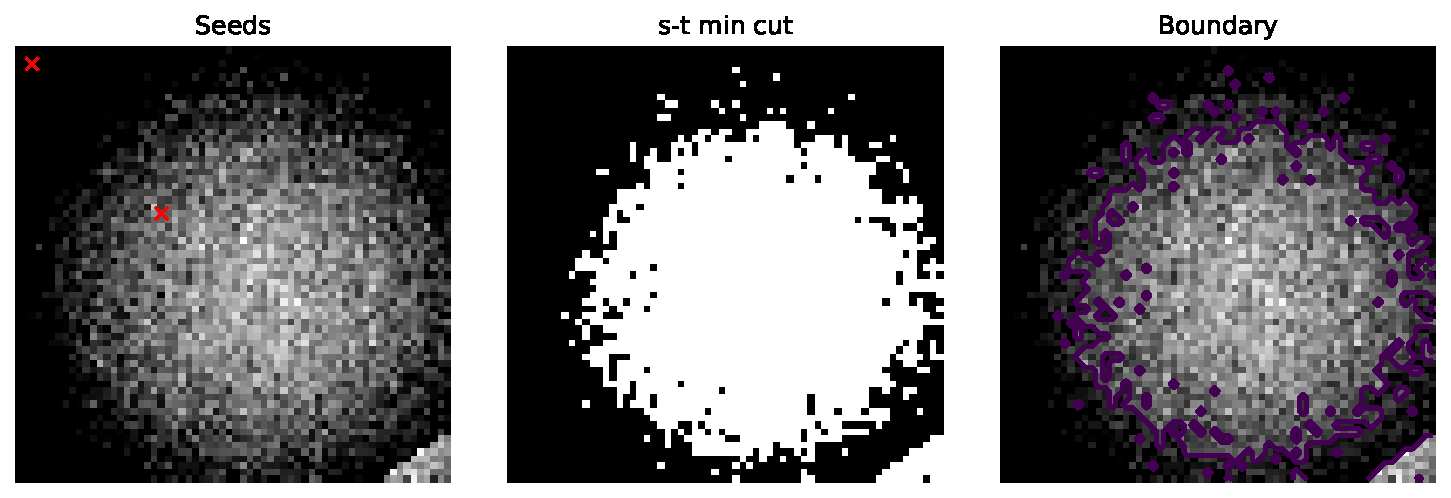
\includegraphics[width=0.87\textwidth]{fig06_graph_cut.pdf}
\caption{قطعه‌بندی تعاملی دودویی با seed و min-cut. unaryها از مدل پیش‌زمینه/پس‌زمینه و pairwiseها از اختلاف همسایه‌ها ساخته می‌شوند.}
\label{fig:graph-cut}
\end{figure}

\begin{algorithmbox}{الگوریتم ۷: graph cut تعاملی}
\begin{enumerate}
\item از scribble یا seed، مدل رنگ پیش‌زمینه و پس‌زمینه را برآورد کنید.
\item unary را به صورت \(-\log p(\vect y_p\mid z_p=k)\) بسازید و seedها را با ظرفیت بزرگ hard-constrain کنید.
\item وزن یال همسایگی را از contrast و فاصله مکانی تعریف کنید.
\item گراف را بسازید و max-flow/min-cut را اجرا کنید.
\item در روش تکراری مانند GrabCut، GMMهای رنگ و برچسب را تناوبی به‌روزرسانی کنید.
\item زمان تعامل، تعداد اصلاح و کیفیت پس از هر prompt را ذخیره کنید.
\end{enumerate}
\end{algorithmbox}

\subsection{چندکلاسه و alpha-expansion}
کمینه‌سازی دقیق Potts چندکلاسه عموماً دشوار است. alpha-expansion در هر حرکت به پیکسل‌ها اجازه می‌دهد برچسب فعلی
را حفظ یا به \(\alpha\) تغییر دهند؛ هر حرکت یک graph cut دودویی است. برای metric pairwise، تقریب دارای کران است.

\subsection{Normalized cut و مسئله مقدار ویژه}
برای گراف وزن‌دار، cut ساده به جداکردن مجموعه کوچک تمایل دارد. معیار
\[
\mathrm{Ncut}(A,B)=\frac{\mathrm{cut}(A,B)}{\mathrm{assoc}(A,V)}
+\frac{\mathrm{cut}(A,B)}{\mathrm{assoc}(B,V)}
\]
قطع را با حجم هر بخش نرمال می‌کند. relaxation پیوسته به مسئله مقدار ویژه تعمیم‌یافته
\[
(\mat D-\mat W)\vect v=\lambda\mat D\vect v
\]
می‌رسد. بردار ویژه دوم اطلاعات دو‌بخشی را می‌دهد. ساخت گراف کامل گران است؛ گراف تنک، Nyström یا superpixel
برای مقیاس‌پذیری استفاده می‌شود.

\subsection{Random walker و توابع هارمونیک}
برای seedهای برچسب‌دار، احتمال اینکه random walk از پیکسل \(p\) نخست به seed کلاس \(k\) برسد، تابع هارمونیک
است. با لاپلاسی گراف \(\Lap=\mat D-\mat W\) و تفکیک گره‌های برچسب‌دار \(M\) و آزاد \(U\):
\[
\begin{bmatrix}
\Lap_{UU}&\Lap_{UM}\\
\Lap_{MU}&\Lap_{MM}
\end{bmatrix}
\begin{bmatrix}\vect{x}_U\\\vect{x}_M\end{bmatrix}=\mathbf{0}
\quad\Rightarrow\quad
\Lap_{UU}\vect{x}_U=-\Lap_{UM}\vect{x}_M.
\]
برای هر کلاس یک دستگاه sparse حل می‌شود و برچسب \(\argmax_k x_{pk}\) است. خروجی probability-like برای تعامل
و uncertainty مفید است.

\begin{figure}[H]
\centering
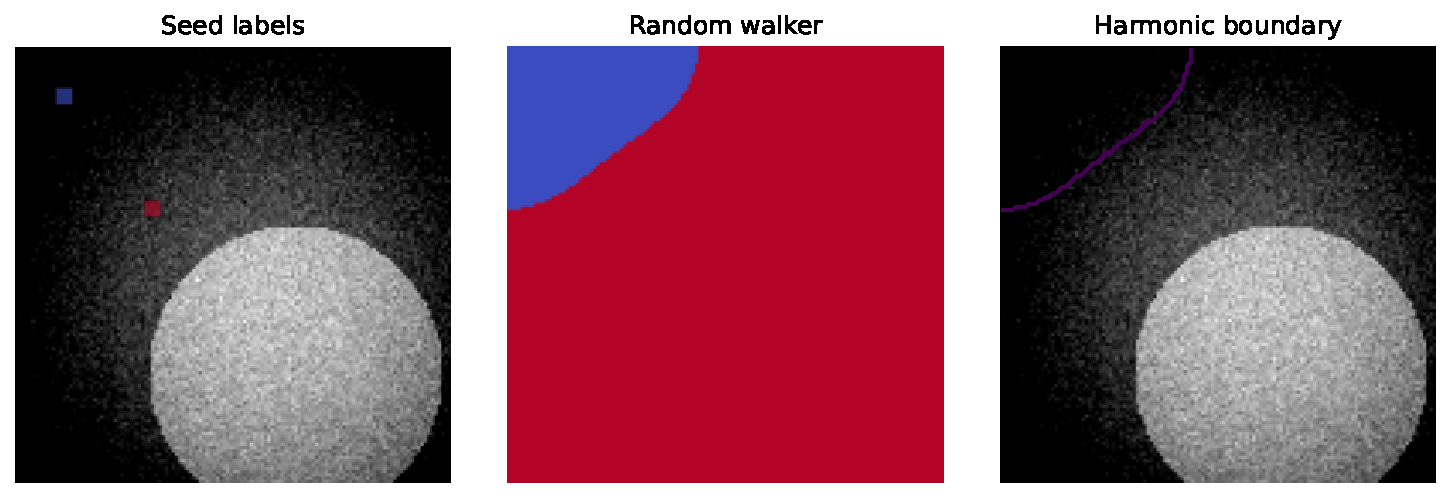
\includegraphics[width=0.86\textwidth]{fig07_random_walker.pdf}
\caption{Random walker: seedها شرط مرزی و لاپلاسی وزن‌دار انتشار احتمال را تعیین می‌کنند. مرز در ناحیه مقاومت بالا قرار می‌گیرد.}
\label{fig:random-walker}
\end{figure}

\begin{proofbox}[اصل کمینه انرژی دیریکله]
راه‌حل هارمونیک random walker کمینه‌کننده
\[
\mathcal E(\vect x)=\frac12\sum_{(p,q)}w_{pq}(x_p-x_q)^2
=\frac12\vect x\trans\Lap\vect x
\]
تحت مقادیر ثابت seed است. مشتق نسبت به \(\vect x_U\) همان دستگاه \(\Lap_{UU}\vect x_U=-\Lap_{UM}\vect x_M\)
را می‌دهد.
\end{proofbox}

\subsection{مقایسه graph cut و random walker}
Graph cut مرز گسسته و مینیمم انرژی Potts می‌دهد؛ random walker پاسخ نرم هارمونیک می‌سازد. graph cut می‌تواند
metrication artifact داشته باشد و به جریمه طول حساس است؛ random walker در ناحیه‌های ضعیف احتمال پخش‌شده و مرز
نرم می‌دهد. انتخاب باید با نوع خطا و تعامل کاربر انجام شود.

\subsection{الگوریتم گرافی Felzenszwalb--Huttenlocher}
این روش یال‌ها را بر اساس تفاوت مرتب و مؤلفه‌ها را union می‌کند اگر تفاوت بین‌مؤلفه‌ای از variation داخلی به علاوه
آستانه وابسته به اندازه کمتر باشد. پیچیدگی تقریباً \(O(E\log E)\) از مرتب‌سازی می‌آید و برای over-segmentation سریع
مفید است، ولی پارامتر scale معنای مستقیم تعداد قطعه ندارد.

\section{ابرپیکسل: کاهش هوشمند تعداد متغیرها}
ابرپیکسل گروه کوچکی از پیکسل‌های مجاور و مشابه است. هدف نهایی لزوماً شیء کامل نیست؛ بلکه جایگزینی میلیون‌ها پیکسل
با چندصد یا چندهزار primitive است که مرزهای مهم را حفظ کنند.

\subsection{SLIC به عنوان k-means محلی}
در فضای \(\vect f_p=[L_p,a_p,b_p,x_p,y_p]\)، فاصله SLIC معمولاً
\[
d_c=\sqrt{(L_p-L_k)^2+(a_p-a_k)^2+(b_p-b_k)^2},
\qquad
d_s=\sqrt{(x_p-x_k)^2+(y_p-y_k)^2},
\]
\[
D=\sqrt{d_c^2+\left(\frac{m}{S}\right)^2d_s^2}
\]
است؛ \(S\approx\sqrt{N/K}\) فاصله شبکه مراکز و \(m\) compactness است. برخلاف k-means عمومی، هر مرکز فقط
در پنجره \(2S\times2S\) جست‌وجو می‌کند؛ از این رو هزینه تقریباً خطی در تعداد پیکسل‌هاست.

\begin{figure}[H]
\centering
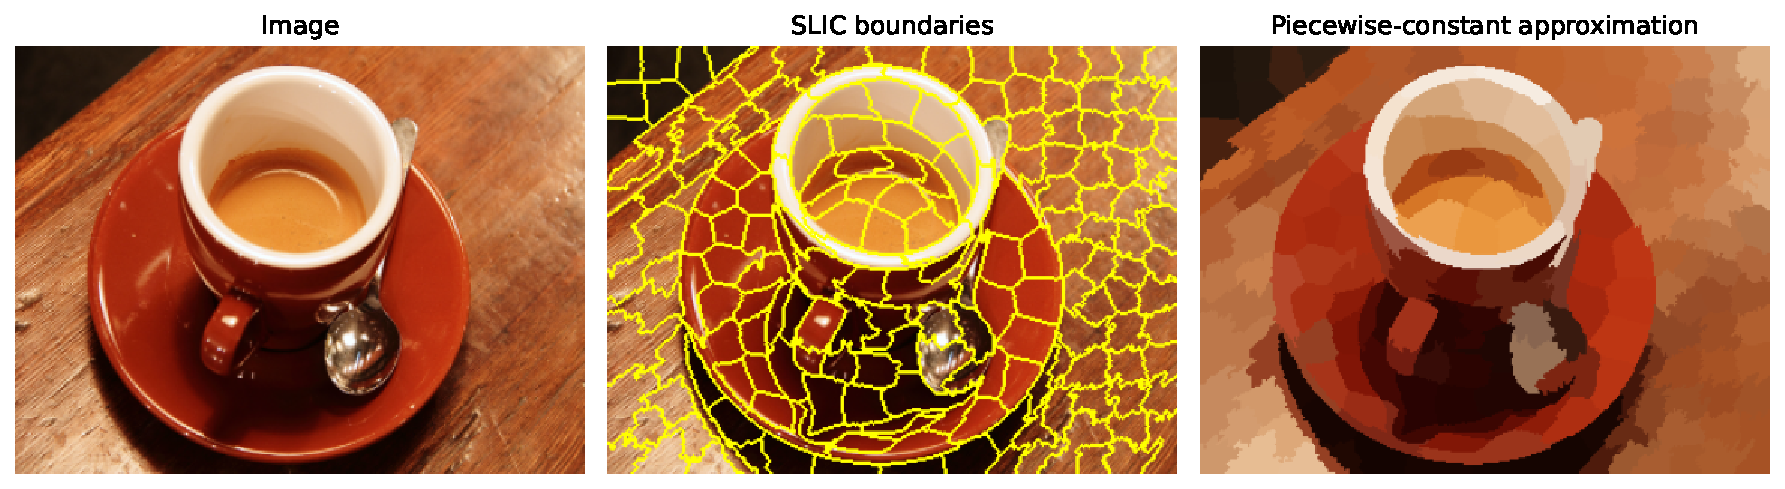
\includegraphics[width=0.95\textwidth]{fig09_slic_superpixels.pdf}
\caption{SLIC، مرز ابرپیکسل و تقریب قطعه‌ای ثابت. افزایش compactness شکل منظم‌تر و adherence مرزی کمتر ایجاد می‌کند.}
\label{fig:slic}
\end{figure}

\begin{algorithmbox}{الگوریتم ۸: SLIC}
\begin{enumerate}
\item تصویر را به فضای رنگ ادراکی تبدیل و \(K\) مرکز روی شبکه با فاصله \(S\) قرار دهید.
\item هر مرکز را در همسایگی کوچک به کمترین گرادیان منتقل کنید تا روی لبه قرار نگیرد.
\item برای هر مرکز فقط پیکسل‌های پنجره \(2S\times2S\) را با فاصله \(D\) ارزیابی کنید.
\item پیکسل را به کمترین فاصله تخصیص و مراکز را میانگین‌گیری کنید.
\item تا تغییر کوچک مراکز یا تعداد iteration ثابت ادامه دهید.
\item در پایان اتصال را صریح enforce و اجزای کوچک را به نزدیک‌ترین همسایه ادغام کنید.
\end{enumerate}
\end{algorithmbox}

\subsection{معیارهای ابرپیکسل}
\begin{itemize}
\item \textbf{Boundary Recall:} چه سهمی از مرز ground truth در فاصله مجاز از مرز ابرپیکسل است؟
\item \textbf{Undersegmentation Error:} یک ابرپیکسل تا چه حد چند ناحیه واقعی را قطع کرده است؟
\item \textbf{Achievable Segmentation Accuracy:} بهترین ماسکی که با نسبت‌دادن یک برچسب به هر ابرپیکسل قابل دستیابی است.
\item \textbf{Compactness و regularity:} شکل و پایداری هندسی، که نباید به قیمت از دست‌دادن مرز مهم بهینه شود.
\end{itemize}
مقایسه باید در تعداد ابرپیکسل برابر یا منحنی کیفیت بر حسب تعداد انجام شود؛ یک نقطه منفرد می‌تواند گمراه‌کننده باشد.

\section{از طبقه‌بندی پیکسل تا شبکه‌های تمام‌کانولوشنی}
\subsection{فرمول‌بندی شبکه}
شبکه \(f_\theta\) logits
\[
\vect a_p=f_\theta(\vect y)_p\in\R^K
\]
و احتمال
\[
p_\theta(z_p=k\mid\vect y)=\frac{e^{a_{pk}}}{\sum_j e^{a_{pj}}}
\]
تولید می‌کند. تفاوت با classifier patch-based آن است که feature extraction مشترک و خروجی dense است. FCN لایه‌های
fully connected را به convolution تبدیل کرد تا تصویر با اندازه متغیر را به نقشه برچسب نگاشت کند.

\subsection{U-Net و مسیر مکان‌یابی}
U-Net یک encoder برای زمینه و decoder برای بازیابی وضوح دارد. skip connection ویژگی کم‌عمق و پرجزئیات را با
ویژگی عمیق و معنایی ترکیب می‌کند. اگر downsampling زیاد باشد، شیء کوچک پیش از decoder حذف می‌شود؛ skip تنها
اطلاعاتی را بازمی‌گرداند که واقعاً در feature map وجود داشته باشد.

\begin{figure}[H]
\centering
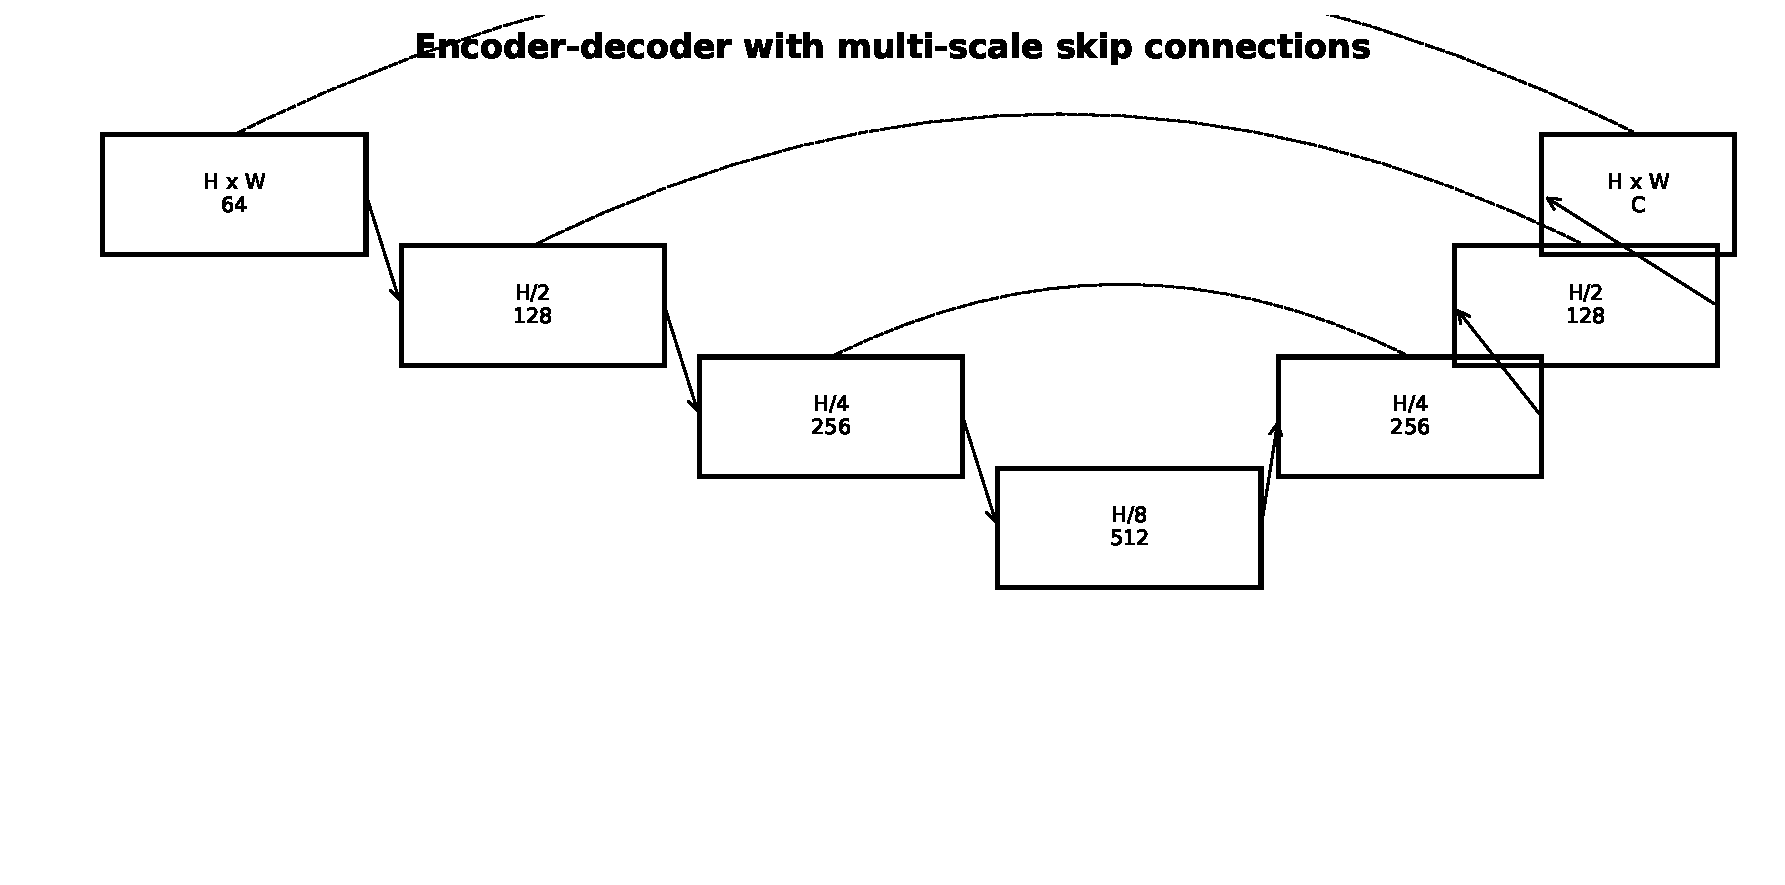
\includegraphics[width=0.92\textwidth]{fig11_unet_architecture.pdf}
\caption{طرح مفهومی encoder--decoder با skipهای چندمقیاسی. اندازه receptive field، stride و حافظه activation سه تصمیم اصلی طراحی‌اند.}
\label{fig:unet}
\end{figure}

\subsection{میدان دید و atrous convolution}
کانولوشن dilated با نرخ \(r\)
\[
y[i]=\sum_k x[i+r k]w[k]
\]
بدون کاهش resolution میدان دید را افزایش می‌دهد. DeepLab از atrous spatial pyramid pooling برای زمینه چندمقیاسی
و decoder برای مرز استفاده می‌کند. نرخ‌های نامناسب می‌توانند gridding artifact ایجاد کنند؛ ترکیب نرخ‌ها و feature
سطوح مختلف راه کاهش آن است.

\subsection{Instance segmentation و Mask R-CNN}
Mask R-CNN یک شاخه ماسک به detector دو مرحله‌ای می‌افزاید. برای هر RoI، ماسک کلاس‌ویژه یا class-agnostic پیش‌بینی
می‌شود. RoIAlign به جای quantization از نمونه‌برداری bilinear استفاده می‌کند تا misalignment فضایی کاهش یابد.
معیار اصلی instance segmentation معمولاً AP ماسک در آستانه‌های مختلف IoU است، نه فقط Dice کلی.

\subsection{Panoptic segmentation}
در panoptic، هر پیکسل یا به یک instance از کلاس thing یا یک ناحیه stuff تعلق دارد. معیار
\[
\mathrm{PQ}=\underbrace{\frac{\sum_{(p,g)\in TP}\IoU(p,g)}{|TP|}}_{\mathrm{SQ}}
\times
\underbrace{\frac{|TP|}{|TP|+\tfrac12|FP|+\tfrac12|FN|}}_{\mathrm{RQ}}
\]
کیفیت قطعه و کیفیت تشخیص را جدا می‌کند. ادغام head معنایی و نمونه‌ای باید تعارض هم‌پوشانی را حل کند.

\subsection{Transformer و پیش‌بینی مجموعه ماسک}
در MaskFormer/Mask2Former، مدل مجموعه‌ای از queryها تولید می‌کند؛ هر query یک embedding کلاس و یک ماسک دارد.
matching دوطرفه Hungarian بین پیش‌بینی و ground truth مسئله permutation را حل می‌کند. masked attention توجه را به
ناحیه ماسک پیش‌بینی‌شده محدود می‌سازد و یک معماری را برای semantic، instance و panoptic مشترک می‌کند.

\begin{futurebox}
در معماری‌های جدید، مرز میان detection و segmentation کم‌رنگ شده است: مدل به جای برچسب مستقل پیکسل، مجموعه‌ای
از mask tokenها، object queryها یا prompt-conditioned masks تولید می‌کند. بنابراین «واحد پیش‌بینی» از پیکسل به
ناحیه و مفهوم انتقال یافته است.
\end{futurebox}

\section{توابع زیان: آنچه آموزش می‌دهیم الزاماً آنچه ارزیابی می‌کنیم نیست}
\subsection{Cross-entropy و وزن‌دهی کلاس}
برای label one-hot:
\[
\mathcal L_{CE}=-\frac1N\sum_p\sum_k y_{pk}\log p_{pk}.
\]
این زیان proper scoring rule است و در حالت ایده‌آل احتمال شرطی را می‌آموزد، اما تعداد زیاد background می‌تواند
گرادیان را غالب کند. weighted CE
\[
\mathcal L_{WCE}=-\frac1N\sum_p w_{z_p}\log p_{p,z_p}
\]
trade-off خطا را تغییر می‌دهد و احتمال خروجی دیگر بدون اصلاح الزاماً کالیبره نیست.

\subsection{Focal loss}
برای مسئله دودویی با \(p_t\) احتمال کلاس درست:
\[
\mathcal L_{focal}=-\alpha_t(1-p_t)^\gamma\log p_t.
\]
نمونه آسان با \(p_t\approx1\) وزن اندک می‌گیرد. \(\gamma\) بزرگ تمرکز بر سخت‌ها را زیاد می‌کند، اما label noise و
مرز مبهم نیز «سخت» هستند و ممکن است بیش‌وزن شوند.

\subsection{Dice و رابطه آن با IoU}
برای مجموعه‌های دودویی \(A,B\):
\[
\Dice(A,B)=\frac{2|A\cap B|}{|A|+|B|},
\qquad
\IoU(A,B)=\frac{|A\cap B|}{|A\cup B|}.
\]
رابطه دقیق
\[
\Dice=\frac{2\IoU}{1+\IoU},
\qquad
\IoU=\frac{\Dice}{2-\Dice}
\]
است؛ بنابراین برای ranking یک مجموعه ثابت یکنوا هستند، ولی averaging per-case باعث برابری کامل گزارش نمی‌شود.
نسخه نرم
\[
\mathcal L_{Dice}=1-\frac{2\sum_p p_py_p+\epsilon}{\sum_p p_p+\sum_p y_p+\epsilon}
\]
نسبت به اندازه foreground سازگارتر است، اما probability calibration را مستقیماً آموزش نمی‌دهد.

\subsection{Tversky و کنترل FP/FN}
\[
T_{\alpha,\beta}=\frac{TP}{TP+\alpha FP+\beta FN},
\qquad
\mathcal L_T=1-T_{\alpha,\beta}.
\]
برای کاربردی که false negative پرهزینه‌تر است، \(\beta>\alpha\) انتخاب می‌شود. این انتخاب باید از هزینه بالینی یا
مهندسی بیاید، نه صرفاً بهترین validation Dice.

\subsection{Lovasz--Softmax}
IoU یک تابع مجموعه‌ای غیرتفاضل‌پذیر است. Lovasz extension برای زیان زیرمدولار Jaccard یک surrogate قطعه‌ای خطی
می‌سازد که خطاها را مرتب و گرادیان را بر اساس تغییر marginal IoU وزن می‌دهد. مزیت هم‌راستایی با mIoU است؛ عیب
پیاده‌سازی حساس به کلاس خالی و تفاوت per-image در برابر per-batch است.

\subsection{زیان مرز، فاصله و توپولوژی}
برای ساختار نازک یا دقت هندسی، CE/Dice کافی نیستند. گزینه‌ها:
\begin{itemize}
\item boundary loss بر اساس distance transform زمین حقیقت؛
\item Hausdorff surrogate برای بدترین فاصله؛
\item سطح یا signed-distance regression؛
\item clDice برای هم‌پوشانی centerline ساختارهای لوله‌ای؛
\item زیان persistence یا Betti برای اتصال و حفره.
\end{itemize}
زیان مرکب
\[
\mathcal L=\lambda_1\mathcal L_{CE}+\lambda_2\mathcal L_{Dice}+\lambda_3\mathcal L_{boundary}
\]
تنها زمانی معنادار است که scale و gradient هر ترم پایش شود؛ ضریب عددی برابر به معنای اثر برابر نیست.

\begin{figure}[H]
\centering
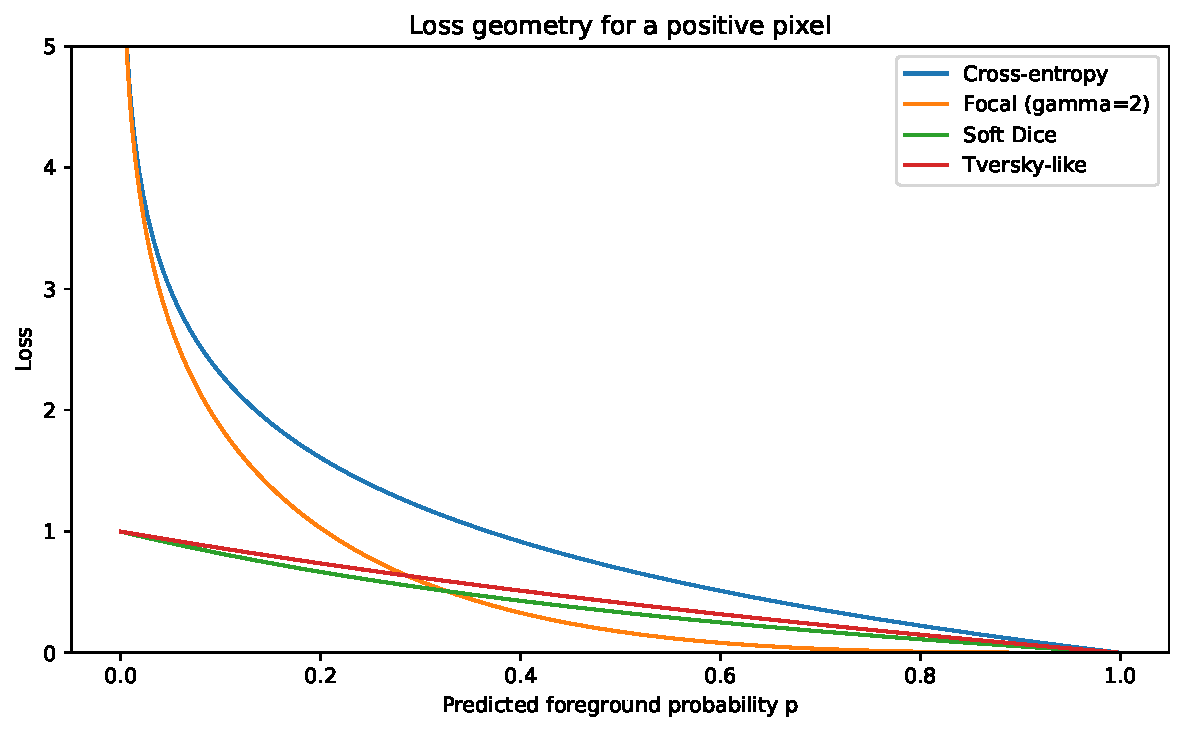
\includegraphics[width=0.72\textwidth]{fig10_loss_geometry.pdf}
\caption{هندسه چند زیان برای یک پیکسل مثبت. زیان‌های overlap به کل ماسک وابسته‌اند و این نمودار تنها شهود موضعی می‌دهد؛ رفتار واقعی به نسبت کلاس و batch بستگی دارد.}
\label{fig:losses}
\end{figure}

\begin{warningbox}
وقتی ground-truth و prediction هر دو خالی‌اند، Dice می‌تواند ۱، ۰ یا undefined تعریف شود. این قرارداد در مسائل
ضایعه نادر نتایج را به شدت تغییر می‌دهد. گزارش باید Dice روی موارد مثبت، نرخ false positive در موارد منفی و میانگین
کل را جدا کند.
\end{warningbox}

\section{داده، برچسب و طراحی آموزش}
\subsection{پروتکل برچسب‌گذاری}
پیش از آموزش باید سند annotation تعریف کند: چه چیزی foreground است؟ مرز نامطمئن چگونه ثبت می‌شود؟ سوراخ،
occlusion، اشیای ناقص در لبه تصویر و پیکسل ignore چه قراردادی دارند؟ توافق بین annotator با Dice یا Cohen's kappa
و تحلیل اختلاف مرزی سنجیده می‌شود. اختلاف انسانی سقف عملی معیار و منبع uncertainty است.

\subsection{تقسیم داده بدون leakage}
در پزشکی، اسلاید، بیمار یا دستگاه باید واحد split باشد؛ در ویدئو، frameهای یک sequence نباید میان train و test پخش
شوند؛ در سنجش‌ازدور، tileهای هم‌پوشان یا مجاور leakage مکانی ایجاد می‌کنند. افزایش مصنوعی تعداد patch جای افزایش
تنوع مستقل را نمی‌گیرد.

\subsection{Patch sampling و عدم‌توازن}
اگر patchها تصادفی باشند، شیء نادر کم دیده می‌شود. sampling می‌تواند بر حضور foreground، مرز، hard example یا
دشواری وزن بگیرد. اما نسبت sampling با prior واقعی deployment متفاوت است و calibration را تغییر می‌دهد. برای
استنباط probability باید این تغییر distribution در نظر گرفته شود.

\subsection{Data augmentation هندسی و فوتومتریک}
تبدیل \(T\) باید همزمان روی تصویر و ماسک اعمال شود. interpolation تصویر می‌تواند bilinear باشد، اما label categorical
به nearest-neighbor نیاز دارد؛ در غیر این صورت labelهای کسری جعلی ساخته می‌شود. transformهای غیرصلب باید با
فیزیک دامنه سازگار باشند. augmentation باید روی train باشد و test-time augmentation جدا گزارش شود.

\subsection{برش تصویر و stitching}
برای تصویر بزرگ، شبکه روی tile اجرا می‌شود. artifact مرز tile با overlap، window weighting و context padding کاهش
می‌یابد. اگر logits پیش از softmax میانگین شوند، با میانگین probability یکسان نیست. قرارداد stitching باید ثابت و
برای همه روش‌ها یکسان باشد.

\subsection{نظارت ضعیف، نیمه‌نظارتی و خودنظارتی}
برچسب ضعیف می‌تواند image-level، point، scribble یا box باشد. pseudo-labeling و consistency regularization از داده
بدون برچسب استفاده می‌کنند:
\[
\mathcal L=\mathcal L_{sup}+	au(t)\,
\norm{f_\theta(T_1(y))-T_1T_2^{-1}f_{\bar\theta}(T_2(y))}^2.
\]
teacher میانگین نمایی و threshold اطمینان خطای confirmation bias را کاهش می‌دهند، اما حذف نمی‌کنند. کیفیت باید
بر حسب مقدار annotation واقعی و هزینه انسانی گزارش شود.

\subsection{Active learning}
معیار انتخاب می‌تواند entropy، margin، disagreement ensemble، diversity یا ترکیب uncertainty و نمایندگی باشد.
در قطعه‌بندی، انتخاب «تصویر» تنها واحد ممکن نیست؛ patch، ناحیه، contour یا prompt نیز می‌تواند query باشد. معیار
علمی مناسب، عملکرد بر حسب دقیقه annotation یا تعداد click است.

\section{عدم‌قطعیت و کالیبراسیون}
\subsection{عدم‌قطعیت aleatoric و epistemic}
Aleatoric از ابهام تصویر و برچسب می‌آید؛ epistemic از کمبود داده و عدم‌قطعیت مدل. ensemble، MC dropout و posterior
تقریبی عمدتاً epistemic را برآورد می‌کنند. entropy softmax هر دو را مخلوط می‌کند و به تنهایی تفکیک‌کننده نیست.

\subsection{کالیبراسیون پیکسلی}
مدل کالیبره برای confidence \(c\) باید تقریباً در \(c\) درصد موارد درست باشد. Expected Calibration Error
\[
\mathrm{ECE}=\sum_{b=1}^{B}\frac{|S_b|}{N}\abs{\mathrm{acc}(S_b)-\mathrm{conf}(S_b)}
\]
به binning حساس است و dominance پس‌زمینه می‌تواند آن را مصنوعی خوب کند. ECE باید per-class، foreground-only و
boundary-aware نیز گزارش شود.

\begin{figure}[H]
\centering
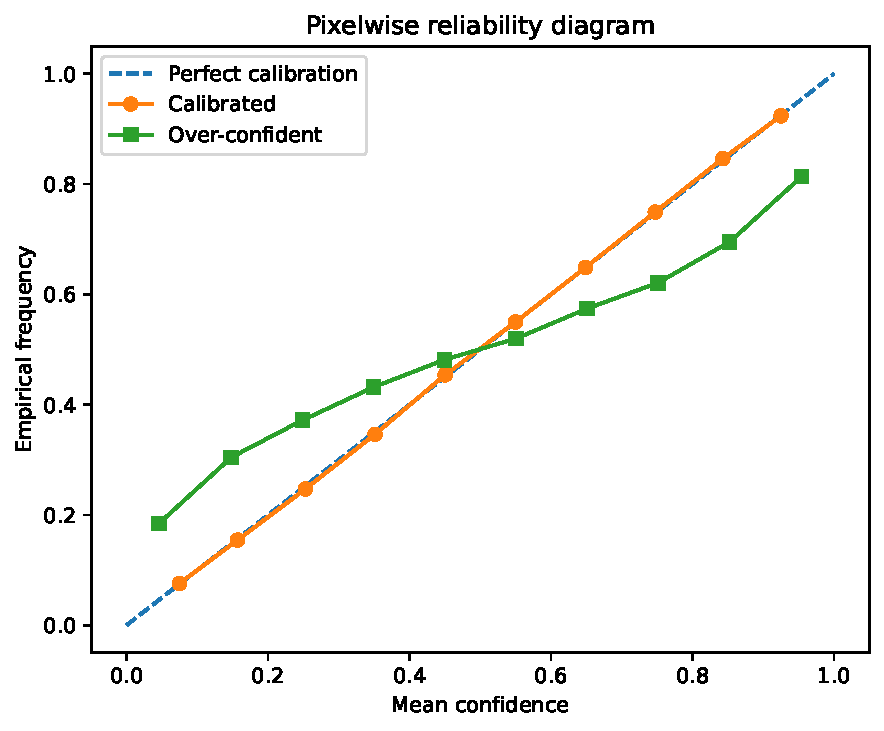
\includegraphics[width=0.68\textwidth]{fig13_segmentation_calibration.pdf}
\caption{نمودار reliability برای خروجی پیکسلی. مدل over-confident می‌تواند Dice بالا ولی probability غیرقابل اعتماد داشته باشد.}
\label{fig:calibration}
\end{figure}

\subsection{Temperature scaling و محدودیت آن}
برای logits \(a\)،
\[
p_k(T)=\softmax(a_k/T).
\]
پارامتر \(T\) روی validation با NLL انتخاب می‌شود. scaling ranking و argmax را عوض نمی‌کند، اما calibration را
بهبود می‌دهد. یک دمای سراسری ممکن است برای کلاس، اندازه شیء و مرزهای متفاوت کافی نباشد.

\subsection{Conformal prediction برای مجموعه برچسب}
با score کالیبراسیون می‌توان برای هر پیکسل مجموعه‌ای از کلاس‌ها ساخت که تحت فرض exchangeability پوشش حاشیه‌ای
تضمین‌شده دارد. اما وابستگی شدید پیکسل‌ها و نیاز به تضمین در سطح شیء یا تصویر، طراحی conformal segmentation را
پیچیده می‌کند؛ تضمین پیکسلی الزاماً تضمین کل ماسک نیست.

\section{مدل‌های بنیادین قطعه‌بندی}
\subsection{SAM: قطعه‌بندی promptable}
SAM مسئله را از «مدل مخصوص کلاس» به «مدل تولید ماسک مشروط به prompt» تغییر داد. اجزای مفهومی آن:
\begin{enumerate}
\item image encoder سنگین که embedding تصویر را یک بار محاسبه می‌کند؛
\item prompt encoder برای point، box و mask؛
\item mask decoder سبک که چند ماسک و برآورد کیفیت تولید می‌کند.
\end{enumerate}
خروجی چندماسکی ابهام prompt را بازتاب می‌دهد: یک click ممکن است به جزء، شیء یا گروه اشاره کند.

\subsection{SAM 2: حافظه جریان برای تصویر و ویدئو}
SAM 2 معماری promptable را به ویدئو گسترش می‌دهد. memory encoder و memory attention اطلاعات فریم‌های گذشته و
promptهای اصلاحی را نگه می‌دارند. ارزیابی ویدئو باید علاوه بر دقت ماسک، drift، بازیابی پس از occlusion، حفظ هویت،
latency و تعداد تعامل را بسنجد.

\subsection{SAM 3: prompt مفهومی}
SAM 3 در ۲۰۲۵ مفهوم promptable concept segmentation را مطرح کرد: متن کوتاه یا exemplar یک مفهوم را تعیین و
مدل همه نمونه‌های مطابق را در تصویر و ویدئو detect، segment و track می‌کند. این گذار مهم است:
\begin{itemize}
\item SAM/SAM 2 عمدتاً می‌پرسند «این ناحیه اشاره‌شده چیست؟»؛
\item SAM 3 می‌پرسد «همه نمونه‌های این مفهوم کجا هستند؟».
\end{itemize}
جداسازی recognition از localization، presence head و tracker حافظه‌دار امکان open-vocabulary mask generation را
فراهم می‌کند. با این حال، مفهوم‌های تخصصی، روابط پیچیده و domain shift هنوز به adaptation و ارزیابی مستقل نیاز دارند.

\begin{figure}[H]
\centering
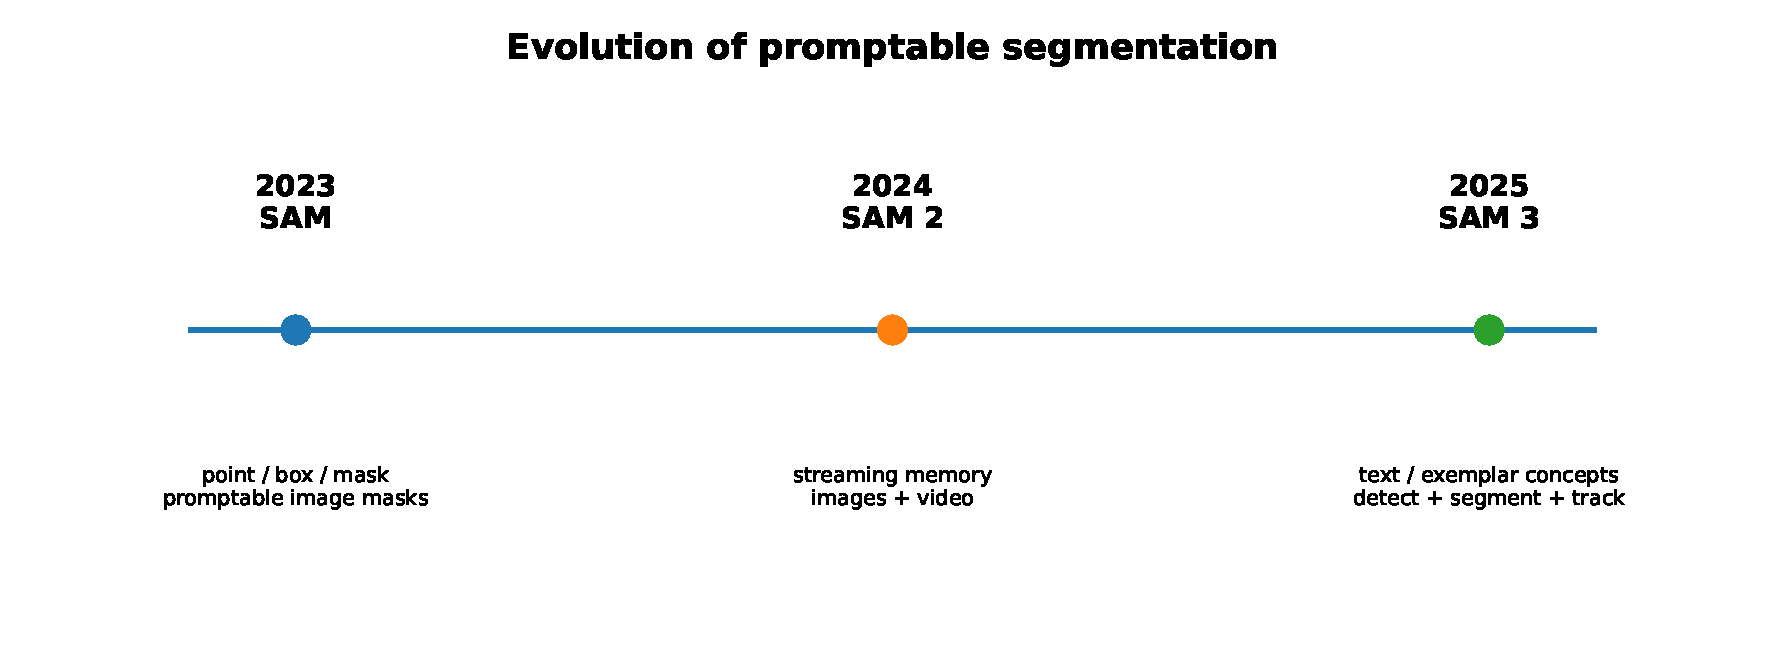
\includegraphics[width=0.88\textwidth]{fig14_sam_evolution.pdf}
\caption{تکامل promptable segmentation از prompt هندسی در تصویر، به حافظه ویدئویی، و سپس prompt مفهومی متنی یا exemplar. شکل، بازطراحی آموزشی است.}
\label{fig:sam-timeline}
\end{figure}

\subsection{Adaptation کم‌هزینه}
راهبردها شامل linear probe، decoder tuning، adapter، LoRA، prompt tuning و distillation هستند. انتخاب لایه‌های قابل
آموزش باید با اندازه داده، فاصله دامنه و حافظه انجام شود. فریز کامل encoder در دامنه‌ای مانند MRI ممکن است ویژگی
نامناسب را تثبیت کند؛ fine-tune کامل با داده کم overfit می‌کند.

\subsection{محدودیت‌ها و ممیزی}
\begin{itemize}
\item مرزهای نازک، اشیای بسیار کوچک و بافت‌های تکراری؛
\item ambiguity معنایی و وابستگی به wording prompt؛
\item domain shift در پزشکی، سنجش‌ازدور و تصویر صنعتی؛
\item confidence غیرکالیبره و نبود تضمین ایمنی؛
\item هزینه حافظه، latency و license/دسترسی مدل؛
\item bias داده و نادیده‌گرفتن اشیای کم‌نماینده؛
\item در ویدئو، drift و باقی‌ماندن ماسک پس از ناپدیدشدن شیء.
\end{itemize}

\begin{researchbox}[مدل بنیادی ابزار است، نه ground truth]
برای ساخت dataset، خروجی SAM می‌تواند annotation را سرعت دهد، اما پذیرش خودکار آن label noise ساختاری و bias مدل
را وارد داده می‌کند. یک حلقه مناسب شامل پیشنهاد مدل، اصلاح انسان، ثبت prompt و زمان، کنترل کیفیت دوگانه و نگهداری
نمونه‌های شکست است.
\end{researchbox}

\section{معیارهای ارزیابی}
\subsection{ماتریس اغتشاش پیکسلی}
برای کلاس دودویی، \(TP,FP,FN,TN\) تعریف می‌شوند. معیارها:
\[
\mathrm{Precision}=\frac{TP}{TP+FP},\qquad
\mathrm{Recall}=\frac{TP}{TP+FN},
\]
\[
\Dice=\frac{2TP}{2TP+FP+FN},
\qquad
\IoU=\frac{TP}{TP+FP+FN}.
\]
Pixel accuracy در foreground کوچک می‌تواند با پیش‌بینی تمام-background بالا باشد؛ balanced accuracy یا per-class
metric لازم است.

\subsection{Macro، micro و وزن‌دهی}
\begin{itemize}
\item macro: میانگین کلاس‌ها با وزن برابر؛ حساس به کلاس نادر؛
\item micro: ابتدا شمارش‌ها جمع و سپس معیار؛ غالب‌شدن کلاس بزرگ؛
\item frequency-weighted: مطابق توزیع پیکسل؛ مناسب برخی کاربردها، ولی نادرها را پنهان می‌کند؛
\item per-image: هر تصویر وزن برابر؛ با dataset-level IoU متفاوت است.
\end{itemize}
همه گزارش‌ها باید نوع averaging را ذکر کنند.

\subsection{مرز و فاصله}
Region IoU برای شیء بزرگ به جابه‌جایی کوچک مرز کم‌حساس است. Boundary IoU نوار مرزی prediction و ground truth را
مقایسه می‌کند. فاصله Hausdorff
\[
H(A,B)=\max\left\{\sup_{a\in A}\inf_{b\in B}d(a,b),
\sup_{b\in B}\inf_{a\in A}d(a,b)\right\}
\]
به یک outlier حساس است؛ HD95 صدک ۹۵ فاصله را گزارش می‌کند. ASSD میانگین فاصله دوطرفه سطح است.

\begin{figure}[H]
\centering
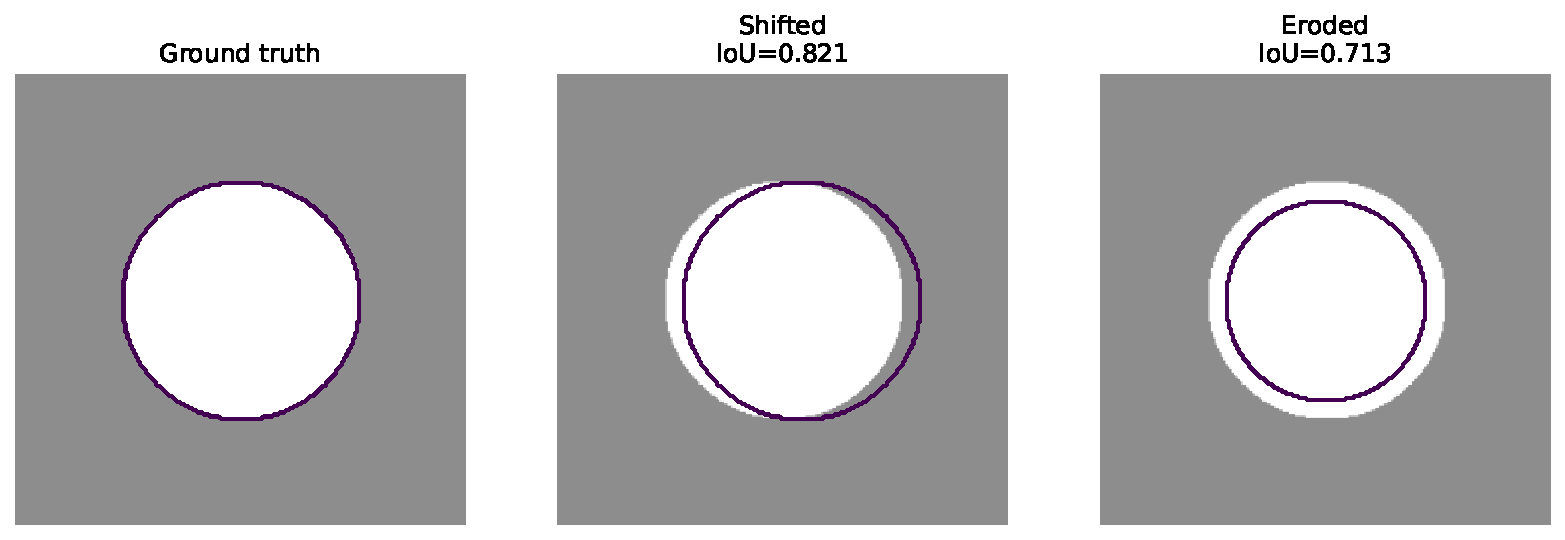
\includegraphics[width=0.82\textwidth]{fig12_region_boundary_metrics.pdf}
\caption{دو خطای هندسی می‌توانند IoU نزدیک ولی پیامد مهندسی متفاوت داشته باشند. ارزیابی باید ناحیه، مرز و در صورت نیاز توپولوژی را همزمان بسنجد.}
\label{fig:metrics}
\end{figure}

\subsection{معیار instance و panoptic}
Instance AP بر matching ماسک‌ها در thresholdهای IoU و منحنی precision--recall است. AJI و PQ برای صحنه‌های چندنمونه‌ای
مفیدند. در شمارش سلول، خطای split/merge باید جدا گزارش شود، زیرا Dice کلی ممکن است ادغام دو سلول را کم‌جریمه کند.

\subsection{توپولوژی و ساختار نازک}
تعداد component، حفره، Betti number، clDice، طول centerline و خطای branch برای رگ، جاده و شبکه عصبی اهمیت دارند.
پس‌پردازش مورفولوژیک ممکن است Dice را بهتر و topology را بدتر کند؛ هر دو باید پیش و پس از post-processing گزارش شوند.

\subsection{آزمون آماری}
برای مقایسه دو مدل روی همان موارد، bootstrap paired روی واحد مستقل (بیمار، صحنه، ویدئو) interval اختلاف را می‌دهد.
میانگین \(\pm\) انحراف معیار روی seedهای تصادفی برای uncertainty آموزش و bootstrap برای uncertainty نمونه‌گیری دو
مفهوم متفاوت‌اند. انتخاب بهترین seed و گزارش آن ممنوع است.

\section{طبقه‌بندی خطا و آزمون فشار}
\begin{figure}[H]
\centering
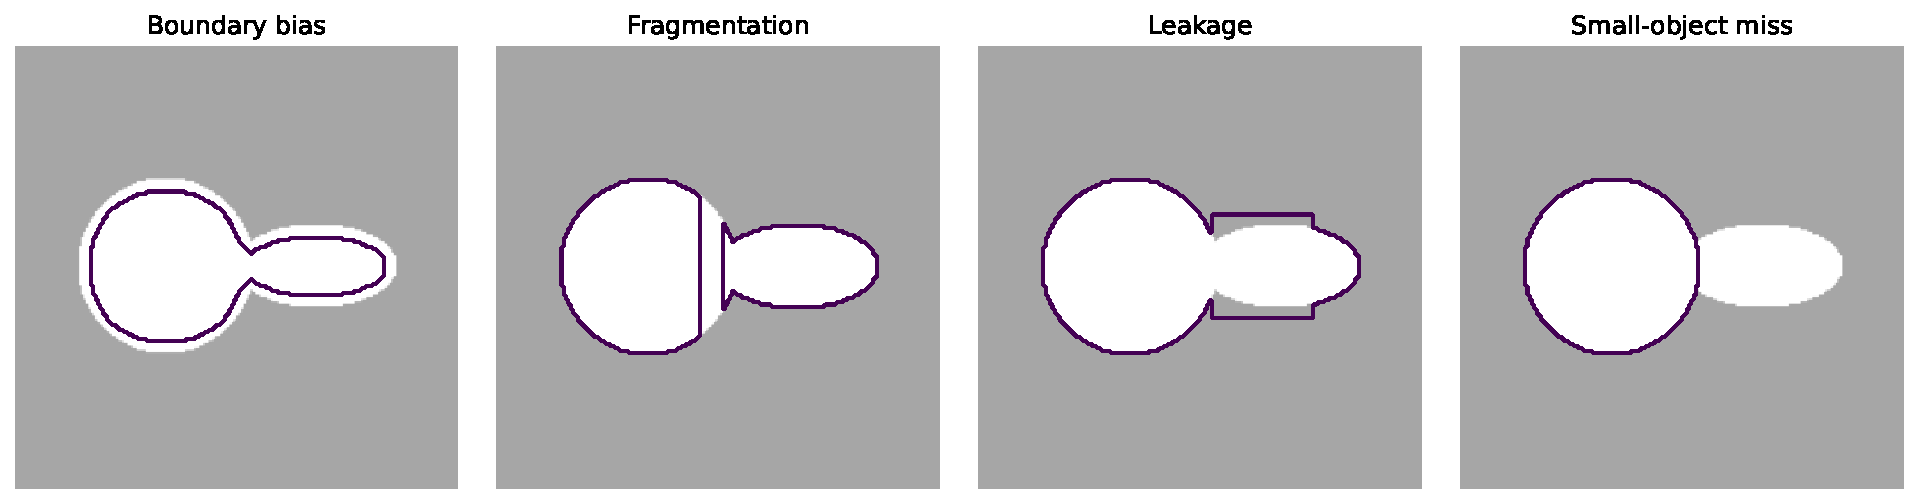
\includegraphics[width=0.94\textwidth]{fig15_failure_modes.pdf}
\caption{چهار خانواده خطای رایج: bias مرز، fragmentation، leakage و حذف شیء کوچک. یک معیار واحد همه را به‌خوبی جدا نمی‌کند.}
\label{fig:failure}
\end{figure}

پروتکل آزمون باید حداقل شامل blur، noise، gamma، compression، تغییر resolution، occlusion، shift دستگاه و کلاس‌های
ناشناخته باشد. robustness را با عملکرد مطلق و افت نسبت به clean گزارش کنید. برای کاربرد واقعی، failure set به‌صورت
دارایی دائمی پروژه نگهداری و در هر نسخه اجرا می‌شود.

\begin{applicationbox}[بازرسی صنعتی]
برای نقص کوچک، معیار pixel accuracy بی‌معناست. ترکیب recall شیء، false alarms per image، localization tolerance،
زمان inference و calibration تصمیم توقف خط تولید لازم است. threshold عملیاتی باید از هزینه false reject و false accept
استخراج شود.
\end{applicationbox}

\begin{applicationbox}[تصویر پزشکی]
گزارش باید patient-level split، HD95/ASSD، موارد خالی، توافق annotator، uncertainty، external validation و اثر خطای
segment بر اندازه‌گیری پایین‌دست را پوشش دهد. نتیجه تصویری زیبا جای تحلیل بالینی را نمی‌گیرد.
\end{applicationbox}

\begin{applicationbox}[سنجش‌ازدور]
اندازه پیکسل زمینی، tile overlap، domain shift جغرافیایی، اشیای بسیار کوچک و مرزهای مبهم اهمیت دارند. split تصادفی
patchهای مجاور معمولاً برآورد خوش‌بینانه می‌دهد؛ split منطقه‌ای یا زمانی معتبرتر است.
\end{applicationbox}

\section{کارگاه پایتون: پیاده‌سازی مرجع و قابل آزمون}
\subsection{Otsu از صفر}
\begin{latin}
\begin{lstlisting}[language=Python]
from __future__ import annotations
import numpy as np


def otsu_threshold(image: np.ndarray, levels: int = 256) -> float:
    """Return an Otsu threshold in the original image scale."""
    x = np.asarray(image, dtype=np.float64)
    if x.ndim != 2 or not np.isfinite(x).all():
        raise ValueError("image must be a finite 2-D array")
    lo, hi = float(x.min()), float(x.max())
    if hi <= lo:
        return lo

    hist, edges = np.histogram(x, bins=levels, range=(lo, hi))
    p = hist.astype(np.float64) / hist.sum()
    centers = 0.5 * (edges[:-1] + edges[1:])
    omega = np.cumsum(p)
    mu = np.cumsum(p * centers)
    mu_total = mu[-1]

    valid = (omega > 0.0) & (omega < 1.0)
    score = np.full(levels, -np.inf)
    numerator = (mu_total * omega[valid] - mu[valid]) ** 2
    score[valid] = numerator / (omega[valid] * (1.0 - omega[valid]))

    maxima = np.flatnonzero(np.isclose(score, np.nanmax(score)))
    idx = int(np.round(maxima.mean()))
    return float(centers[idx])
\end{lstlisting}
\end{latin}

\subsection{آستانه Sauvola با کنترل نوع داده}
\begin{latin}
\begin{lstlisting}[language=Python]
import numpy as np
from scipy.ndimage import uniform_filter


def sauvola_mask(image, window=41, k=0.2, r=None, foreground="bright"):
    x = np.asarray(image, dtype=np.float64)
    if x.ndim != 2 or window < 3 or window % 2 == 0:
        raise ValueError("window must be an odd integer >= 3")
    mean = uniform_filter(x, size=window, mode="reflect")
    mean_sq = uniform_filter(x * x, size=window, mode="reflect")
    std = np.sqrt(np.maximum(mean_sq - mean * mean, 0.0))
    if r is None:
        r = 0.5 * (np.percentile(x, 99.5) - np.percentile(x, 0.5))
        r = max(float(r), np.finfo(float).eps)
    threshold = mean * (1.0 + k * (std / r - 1.0))
    return (x > threshold) if foreground == "bright" else (x < threshold)
\end{lstlisting}
\end{latin}

\subsection{رشد ناحیه با صف و آمار آنلاین}
\begin{latin}
\begin{lstlisting}[language=Python]
from collections import deque
import numpy as np


def region_grow(image, seed, tolerance, connectivity=4):
    x = np.asarray(image, dtype=np.float64)
    h, w = x.shape
    r0, c0 = seed
    if not (0 <= r0 < h and 0 <= c0 < w):
        raise ValueError("seed is outside image")
    offsets = [(-1, 0), (1, 0), (0, -1), (0, 1)]
    if connectivity == 8:
        offsets += [(-1, -1), (-1, 1), (1, -1), (1, 1)]

    accepted = np.zeros((h, w), dtype=bool)
    visited = np.zeros((h, w), dtype=bool)
    q = deque([(r0, c0)])
    visited[r0, c0] = True
    mean, count = float(x[r0, c0]), 0

    while q:
        r, c = q.popleft()
        if abs(float(x[r, c]) - mean) > tolerance:
            continue
        accepted[r, c] = True
        count += 1
        mean += (float(x[r, c]) - mean) / count
        for dr, dc in offsets:
            rr, cc = r + dr, c + dc
            if 0 <= rr < h and 0 <= cc < w and not visited[rr, cc]:
                visited[rr, cc] = True
                q.append((rr, cc))
    return accepted
\end{lstlisting}
\end{latin}

\subsection{GMM و نگاشت مسئولیت}
\begin{latin}
\begin{lstlisting}[language=Python]
import numpy as np
from sklearn.mixture import GaussianMixture


def gmm_segment(image, n_components=3, spatial_weight=0.0, seed=0):
    x = np.asarray(image, dtype=np.float64)
    h, w = x.shape[:2]
    color = x[..., None] if x.ndim == 2 else x
    yy, xx = np.mgrid[:h, :w]
    features = color.reshape(-1, color.shape[-1])
    if spatial_weight > 0:
        space = np.column_stack((xx.ravel() / w, yy.ravel() / h))
        features = np.column_stack((features, spatial_weight * space))
    features = (features - features.mean(0)) / (features.std(0) + 1e-8)
    model = GaussianMixture(
        n_components=n_components,
        covariance_type="full",
        reg_covar=1e-5,
        n_init=5,
        random_state=seed,
    ).fit(features)
    responsibilities = model.predict_proba(features).reshape(h, w, n_components)
    labels = responsibilities.argmax(axis=-1)
    uncertainty = -(responsibilities * np.log(responsibilities + 1e-12)).sum(-1)
    return labels, uncertainty, model
\end{lstlisting}
\end{latin}

\subsection{Random walker و Chan--Vese با scikit-image}
\begin{latin}
\begin{lstlisting}[language=Python]
import numpy as np
from skimage.segmentation import random_walker, morphological_chan_vese


def random_walker_from_seeds(image, foreground, background, beta=130):
    markers = np.zeros(image.shape, dtype=np.int32)
    markers[np.asarray(background, bool)] = 1
    markers[np.asarray(foreground, bool)] = 2
    if not np.any(markers == 1) or not np.any(markers == 2):
        raise ValueError("both foreground and background seeds are required")
    return random_walker(image, markers, beta=beta, mode="cg_j") == 2


def chan_vese_segment(image, iterations=150, smoothing=2):
    return morphological_chan_vese(
        np.asarray(image, dtype=float),
        num_iter=iterations,
        init_level_set="checkerboard",
        smoothing=smoothing,
    )
\end{lstlisting}
\end{latin}

\subsection{معیارهای مقاوم به ماسک خالی}
\begin{latin}
\begin{lstlisting}[language=Python]
import numpy as np


def binary_metrics(pred, target, empty_value=1.0):
    p = np.asarray(pred, bool)
    y = np.asarray(target, bool)
    if p.shape != y.shape:
        raise ValueError("shape mismatch")
    tp = np.logical_and(p, y).sum()
    fp = np.logical_and(p, ~y).sum()
    fn = np.logical_and(~p, y).sum()
    union = tp + fp + fn
    denom = 2 * tp + fp + fn
    return {
        "iou": float(empty_value if union == 0 else tp / union),
        "dice": float(empty_value if denom == 0 else 2 * tp / denom),
        "precision": float(1.0 if tp + fp == 0 else tp / (tp + fp)),
        "recall": float(1.0 if tp + fn == 0 else tp / (tp + fn)),
    }
\end{lstlisting}
\end{latin}

\subsection{اسکلت فشرده U-Net در PyTorch}
\begin{latin}
\begin{lstlisting}[language=Python]
import torch
from torch import nn


class ConvBlock(nn.Module):
    def __init__(self, c_in, c_out):
        super().__init__()
        self.net = nn.Sequential(
            nn.Conv2d(c_in, c_out, 3, padding=1, bias=False),
            nn.BatchNorm2d(c_out), nn.ReLU(inplace=True),
            nn.Conv2d(c_out, c_out, 3, padding=1, bias=False),
            nn.BatchNorm2d(c_out), nn.ReLU(inplace=True),
        )
    def forward(self, x):
        return self.net(x)


class SmallUNet(nn.Module):
    def __init__(self, in_channels=1, classes=2, base=32):
        super().__init__()
        self.e1 = ConvBlock(in_channels, base)
        self.e2 = ConvBlock(base, 2 * base)
        self.b = ConvBlock(2 * base, 4 * base)
        self.pool = nn.MaxPool2d(2)
        self.up2 = nn.ConvTranspose2d(4 * base, 2 * base, 2, stride=2)
        self.d2 = ConvBlock(4 * base, 2 * base)
        self.up1 = nn.ConvTranspose2d(2 * base, base, 2, stride=2)
        self.d1 = ConvBlock(2 * base, base)
        self.head = nn.Conv2d(base, classes, 1)

    def forward(self, x):
        e1 = self.e1(x)
        e2 = self.e2(self.pool(e1))
        b = self.b(self.pool(e2))
        d2 = self.d2(torch.cat([self.up2(b), e2], dim=1))
        d1 = self.d1(torch.cat([self.up1(d2), e1], dim=1))
        return self.head(d1)
\end{lstlisting}
\end{latin}

\begin{warningbox}
کد آموزشی کوتاه جای pipeline تولیدی را نمی‌گیرد. mixed precision، distributed training، deterministic mode، checkpoint،
normalization، logging، validation بدون leakage و مدیریت ماسک ignore باید در پروژه واقعی اضافه شوند.
\end{warningbox}

\section{الگوریتم آموزش و ارزیابی شبکه}
\begin{algorithmbox}{الگوریتم ۹: آموزش قابل بازتولید شبکه قطعه‌بندی}
\begin{enumerate}
\item واحد مستقل split را تعریف و train/validation/test را پیش از هر tuning تثبیت کنید.
\item transform مشترک تصویر--ماسک را با interpolation صحیح بسازید.
\item seed همه کتابخانه‌ها، نسخه محیط و hash داده را ذخیره کنید.
\item loss اصلی و auxiliary را تعریف و magnitude و gradient آنها را log کنید.
\item در هر epoch، metricهای per-class، موارد خالی، مرز و calibration را روی validation محاسبه کنید.
\item checkpoint را بر معیار از پیش تعیین‌شده، نه انتخاب پسینی بهترین چند معیار، ذخیره کنید.
\item پس از پایان tuning، test را فقط یک بار اجرا و bootstrap paired را روی واحد مستقل محاسبه کنید.
\item نمونه‌های شکست، latency، حافظه و threshold عملیاتی را همراه وزن مدل منتشر کنید.
\end{enumerate}
\end{algorithmbox}

\begin{algorithmbox}{الگوریتم ۱۰: پالایش تعاملی promptable}
\begin{enumerate}
\item prompt اولیه point یا box را از کاربر یا detector بگیرید.
\item چند ماسک و کیفیت پیش‌بینی‌شده را تولید و بهترین را نمایش دهید.
\item کاربر بزرگ‌ترین ناحیه خطا را با click مثبت/منفی یا scribble اصلاح کند.
\item prompt جدید و ماسک قبلی را به decoder بدهید و زمان تعامل را ثبت کنید.
\item تا رسیدن به IoU هدف یا سقف تعامل ادامه دهید.
\item منحنی کیفیت بر حسب click و زمان annotation را گزارش کنید.
\end{enumerate}
\end{algorithmbox}

\section{آزمایش‌های پیشنهادی فصل}
\subsection{آزمایش ۱: مرز اعتبار Otsu}
دو گاوسی با فاصله میانگین، نسبت کلاس و واریانس متفاوت بسازید. threshold بیزی، Otsu و minimum-error را از نظر
خطای طبقه‌بندی و bias آستانه مقایسه کنید. سپس spatial arrangement را تغییر دهید و نشان دهید Otsu به آن حساس نیست.

\subsection{آزمایش ۲: روشنایی ناهمگن}
تصویر سند مصنوعی با میدان روشنایی polynomial و نویز بسازید. Otsu، background subtraction، Niblack و Sauvola را
روی شبکه‌ای از اندازه پنجره و \(k\) ارزیابی کنید. heatmap پارامتر و پایداری را گزارش کنید.

\subsection{آزمایش ۳: رشد ناحیه و ترتیب}
seed، tolerance، اتصال و ساختار صف را تغییر دهید. leakage، تعداد مؤلفه و زمان را بسنجید. نسخه mean-updating را با
مدل ثابت seed و مدل مقاوم median مقایسه کنید.

\subsection{آزمایش ۴: GMM و ویژگی مکانی}
GMM شدت‌محور، رنگ‌محور و رنگ+مکان را روی تصاویر با اشیای هم‌رنگ در مکان‌های جدا مقایسه کنید. entropy مسئولیت و
اثر covariance full/diag را گزارش کنید.

\subsection{آزمایش ۵: graph cut در برابر random walker}
برای seed یکسان، \(\beta\) و \(\lambda\) را تغییر دهید. کیفیت مرز، ناحیه اطمینان، زمان حل و حساسیت به seed اشتباه
را تحلیل کنید.

\subsection{آزمایش ۶: Chan--Vese زیر مدل‌های مختلف}
تصاویر piecewise-constant، روشنایی گرادیانی و بافت‌دار بسازید. اثر initialization، \(\mu\)، smoothing و تعداد iteration
را بر انرژی و IoU گزارش کنید.

\subsection{آزمایش ۷: ابرپیکسل}
SLIC را روی تعداد ابرپیکسل و compactness مختلف اجرا کنید. Boundary Recall، Undersegmentation Error، ASA، زمان و
حافظه را به صورت منحنی گزارش کنید.

\subsection{آزمایش ۸: loss و عدم‌توازن}
U-Net کوچک را با CE، weighted CE، Dice، CE+Dice، focal و Tversky روی نسبت foregroundهای مختلف آموزش دهید. علاوه
بر Dice، precision/recall، calibration، gradient norm و عملکرد روی ماسک خالی را گزارش کنید.

\subsection{آزمایش ۹: کیفیت مرز}
دو مدل با region IoU مشابه ولی decoder متفاوت بسازید. Boundary IoU، HD95، ASSD و خطای اندازه‌گیری مساحت/محیط را
مقایسه کنید.

\subsection{آزمایش ۱۰: promptable segmentation}
SAM-family یا مدل promptable در دسترس را با point، box و mask prompt روی چند دامنه اجرا کنید. کیفیت بر حسب تعداد
click، latency، object size، domain و failure type گزارش شود. هیچ نتیجه‌ای بدون ذکر checkpoint و license معتبر نیست.

\subsection{آزمایش ۱۱: تعمیم خارج از توزیع}
مدل را روی یک مرکز، حسگر یا فصل آموزش و روی مرکز/حسگر/فصل دیگر ارزیابی کنید. افت clean-to-OOD، calibration و
uncertainty-error correlation را گزارش کنید.

\subsection{آزمایش ۱۲: اثر قطعه‌بندی بر وظیفه پایین‌دست}
ماسک را برای اندازه‌گیری، شمارش، classification یا کنترل ربات استفاده کنید. نشان دهید بهبود Dice همیشه بهبود وظیفه
پایین‌دست نیست؛ sensitivity وظیفه به انواع خطا را استخراج کنید.

\section{پروتکل گزارش حرفه‌ای}
\begin{longtable}{p{37mm}p{102mm}}
\toprule
جزء گزارش & حداقل اطلاعات لازم \\
\midrule
داده & منبع، license، واحد split، تعداد مستقل، توزیع کلاس، resolution، modality، حذف‌ها \\
برچسب & دستورالعمل، annotator، توافق، ignore، ماسک خالی، کنترل کیفیت \\
پیش‌پردازش & normalization، resize، crop، رنگ، interpolation، padding \\
مدل & معماری، backbone، checkpoint، تعداد پارامتر، receptive field، ورودی \\
آموزش & optimizer، schedule، batch، epoch، seed، augmentation، loss و ضرایب \\
انتخاب مدل & معیار validation و قانون early stopping از پیش تعیین‌شده \\
ارزیابی & averaging، threshold، post-processing، CI، test مستقل، موارد خالی \\
مهندسی & سخت‌افزار، latency batch=1، throughput، peak memory، انرژی در صورت اهمیت \\
شکست & نمونه‌های کیفی انتخاب‌نشده، taxonomy خطا، OOD، corruption، prompt sensitivity \\
بازتولید & کد، environment lock، hash داده، command line، log و checkpoint \\
\bottomrule
\end{longtable}

\section{تمرین‌های نظری و اثباتی}
\begin{enumerate}
\item آستانه بیزی دو گاوسی با واریانس نابرابر و هزینه نامتقارن را استخراج و تعداد نقاط تصمیم را تحلیل کنید.
\item برابری کمینه \(\sigma_w^2\) و بیشینه \(\sigma_b^2\) در Otsu را اثبات کنید.
\item فرمول هزینه بازه \(C(a,b)\) را با سه مجموع تجمعی برای Multi-Otsu استخراج کنید.
\item نشان دهید هر iteration Lloyd تابع هدف k-means را افزایش نمی‌دهد.
\item با نابرابری Jensen، گام E در EM و lower bound درست‌نمایی را توضیح دهید.
\item معادله اویلر--لاگرانژ Chan--Vese را با تقریب نرم Heaviside استخراج کنید.
\item شرط زیرمدولار graph cut را برای Potts بررسی و یک pairwise غیرقابل نمایش بسازید.
\item دستگاه random walker را از کمینه انرژی دیریکله به دست آورید.
\item مسئله relaxed normalized cut را از Rayleigh quotient استخراج کنید.
\item پیچیدگی SLIC را با محدودشدن جست‌وجوی هر مرکز به \(2S\times2S\) تحلیل کنید.
\item رابطه Dice و IoU را اثبات و اثر averaging per-image را با مثال نقض نشان دهید.
\item گرادیان soft Dice نسبت به probability یک پیکسل را استخراج و coupling بین پیکسل‌ها را نشان دهید.
\item یک مثال بسازید که pixel accuracy بالا و IoU foreground صفر باشد.
\item PQ را برای سه prediction شامل split، merge و false positive محاسبه کنید.
\item توضیح دهید چرا temperature scaling argmax را عوض نمی‌کند.
\item یک زیان مرکب برای رگ پیشنهاد و اثر هر ترم را از نظر گرادیان تحلیل کنید.
\item برای interactive segmentation، معیار Area Under NoC Curve را تعریف و مزیت آن را نسبت به IoU یک prompt بیان کنید.
\item یک پروتکل conformal برای پوشش سطح شیء پیشنهاد و تفاوت آن با پوشش پیکسلی را تحلیل کنید.
\end{enumerate}

\section{پروژه‌های پایان فصل}
\subsection{پروژه A: آزمایشگاه جامع آستانه‌گذاری}
یک بسته Python با Otsu، Multi-Otsu، Kittler، Triangle، Niblack، Sauvola و hysteresis بسازید. همه روش‌ها باید API
یکسان، تست واحد، benchmark، پشتیبانی uint8/uint16/float و گزارش stability داشته باشند.

\subsection{پروژه B: قطعه‌بندی تعاملی کلاسیک و بنیادی}
Graph cut، random walker و یک SAM-family model را با prompt یکسان مقایسه کنید. معیار اصلی کیفیت بر حسب click و
زمان کاربر باشد؛ failure prompt و domain shift را دسته‌بندی کنید.

\subsection{پروژه C: قطعه‌بندی پزشکی با عدم‌قطعیت}
یک U-Net سه‌بعدی یا دوبعدی را با ensemble آموزش دهید. Dice، HD95، calibration، uncertainty-error، external test و
اثر بر اندازه‌گیری بالینی را گزارش کنید.

\subsection{پروژه D: قطعه‌بندی ناحیه‌ای هیبرید}
ابتدا SLIC یا watershed، سپس GNN/CRF روی region adjacency graph اجرا کنید. کیفیت، حافظه و سرعت را با شبکه dense
مقایسه کنید.

\subsection{پروژه E: مدل بنیادی برای تولید داده}
یک حلقه annotation با پیشنهاد SAM، اصلاح انسان، کنترل کیفیت و active learning بسازید. زمان annotation، نرخ اصلاح،
bias کلاس و سود واقعی نسبت به برچسب‌گذاری دستی را اندازه بگیرید.

\subsection{پروژه F: قطعه‌بندی توپولوژی‌آگاه}
برای رگ، جاده یا crack، CE+Dice را با boundary و clDice/topology loss مقایسه کنید. Betti error، centerline distance و
کارایی پایین‌دست را وارد ارزیابی کنید.

\section{پرامپت پیشنهادی برای Codex}
\begin{latin}
\begin{lstlisting}[language={}]
Build a fully reproducible Python research package for Chapter 8, "Image
Segmentation: From Thresholding to Foundation Models".

Implement from scratch where educationally useful:
- Bayesian two-class thresholding with asymmetric costs;
- stable Otsu and dynamic-programming multi-Otsu;
- integral-image local mean/variance, Niblack and Sauvola;
- queue-based region growing with 4/8 connectivity;
- k-means, GMM-EM with log-sum-exp and fuzzy c-means;
- binary s-t graph cut and random walker;
- Chan-Vese level set with energy logging;
- SLIC superpixels and boundary-recall/undersegmentation metrics;
- binary and multiclass segmentation metrics, Boundary IoU, HD95, ASSD,
  calibration and paired bootstrap confidence intervals;
- a compact PyTorch U-Net training pipeline with CE, focal, Dice, Tversky,
  Lovasz and boundary-aware losses.

Add wrappers, not fake reimplementations, for current promptable segmentation
models when weights and licenses are available. Record model name, checkpoint,
commit, license, prompt type, inference device and latency. Never download
weights silently and never fabricate benchmark results.

Research requirements:
1. Use synthetic data with analytic ground truth plus at least three public
   datasets from different domains (documents, natural images, medical,
   remote sensing or industrial inspection).
2. Prevent patient/scene/video/tile leakage using group-aware splits.
3. Save every configuration, random seed, environment, command line and input
   hash. Produce CSV, JSON and publication-quality PDF figures.
4. Evaluate region, boundary, instance/topology and calibration metrics.
5. Include robustness tests for blur, noise, JPEG, gamma, scale, occlusion and
   domain shift.
6. Report mean and standard deviation across training seeds and paired
   bootstrap confidence intervals across independent test units.
7. Benchmark runtime and peak memory on CPU and GPU when available.
8. Add unit and property tests for empty masks, ignored labels, label remapping,
   connectivity, deterministic transforms and metric edge cases.
9. Generate a failure gallery automatically, without cherry-picking, by
   sorting cases using predeclared error criteria.
10. Provide one command that regenerates all chapter figures and tables.
\end{lstlisting}
\end{latin}

\section{تقسیم پیشنهادی ویدئوهای ۱۵ دقیقه‌ای}
\begin{longtable}{p{12mm}p{115mm}}
\toprule
بخش & موضوع \\
\midrule
1 & تعریف قطعه‌بندی و taxonomy وظایف \\
2 & تصمیم بیزی و نسبت درست‌نمایی \\
3 & آستانه گاوسی با هزینه نامتقارن \\
4 & استخراج Otsu \\
5 & پیاده‌سازی پایدار Otsu \\
6 & Multi-Otsu و برنامه‌ریزی پویا \\
7 & entropy، minimum error و Triangle \\
8 & مدل روشنایی ناهمگن \\
9 & تصویر انتگرالی و آستانه محلی \\
10 & Niblack، Sauvola و انتخاب پنجره \\
11 & hysteresis و threshold چندکاناله \\
12 & رشد ناحیه و seed \\
13 & الگوریتم صف‌محور و پیچیدگی \\
14 & split--merge و watershed نشان‌محور \\
15 & k-means در فضای رنگ--مکان \\
16 & استخراج EM برای GMM \\
17 & fuzzy c-means و mean shift \\
18 & MRF Potts و ساختار مکانی \\
19 & تابع Mumford--Shah \\
20 & استخراج Chan--Vese \\
21 & level set و curvature \\
22 & geodesic contour و مدل‌های محلی \\
23 & انرژی graph cut و گراف s--t \\
24 & شرط زیرمدولار و max-flow/min-cut \\
25 & alpha-expansion و چندکلاسه \\
26 & normalized cut و مسئله مقدار ویژه \\
27 & random walker و لاپلاسی گراف \\
28 & مقایسه graph cut و random walker \\
29 & SLIC و فاصله رنگ--مکان \\
30 & معیارهای ابرپیکسل \\
31 & FCN و طبقه‌بندی dense \\
32 & U-Net و skip connection \\
33 & atrous convolution و DeepLab \\
34 & Mask R-CNN و instance segmentation \\
35 & panoptic segmentation و PQ \\
36 & Transformer، MaskFormer و Mask2Former \\
37 & cross-entropy و عدم‌توازن \\
38 & focal، Dice و Tversky \\
39 & Lovasz و زیان مرزی \\
40 & topology loss و ساختار نازک \\
41 & برچسب‌گذاری، split و leakage \\
42 & patch sampling، augmentation و stitching \\
43 & نیمه‌نظارتی و active learning \\
44 & عدم‌قطعیت و calibration \\
45 & SAM و promptable masks \\
46 & SAM 2 و حافظه ویدئویی \\
47 & SAM 3 و prompt مفهومی \\
48 & adaptation مدل بنیادی و محدودیت‌ها \\
49 & IoU، Dice و averaging \\
50 & Boundary IoU، HD95 و ASSD \\
51 & instance AP و panoptic PQ \\
52 & ارزیابی توپولوژی و calibration \\
53 & آزمون آماری و paired bootstrap \\
54 & کارگاه کدنویسی کلاسیک \\
55 & کارگاه U-Net و loss \\
56 & طراحی failure gallery و robustness \\
57 & پروژه‌های حوزه پزشکی، صنعتی و سنجش‌ازدور \\
58 & مرور مقاله‌های مرزی و جمع‌بندی \\
\bottomrule
\end{longtable}

\section{جمع‌بندی و پل به فصل نهم}
\begin{summarybox}
\begin{enumerate}
\item قطعه‌بندی یک تصمیم وابسته به هدف است؛ «ناحیه درست» بدون تعریف کاربرد معنا ندارد.
\item آستانه‌گذاری حالت خاص تصمیم بیزی است و Otsu جدایی واریانسی شدت را بدون استفاده از مکان بهینه می‌کند.
\item روشنایی ناهمگن نیازمند تصحیح photometric یا آستانه تابع مکان است؛ تصویر انتگرالی محاسبه محلی را خطی می‌کند.
\item رشد ناحیه اتصال و seed را وارد تصمیم می‌کند، ولی به predicate، ترتیب و leakage حساس است.
\item k-means و GMM مدل ظاهر می‌سازند؛ ساختار مکانی باید با ویژگی مکان یا prior گرافی اضافه شود.
\item Mumford--Shah و Chan--Vese قطعه‌بندی را به کمینه‌سازی fidelity، همواری و طول مرز تبدیل می‌کنند.
\item graph cut برای انرژی دودویی زیرمدولار مینیمم سراسری و random walker راه‌حل هارمونیک نرم تولید می‌کند.
\item superpixel تعداد متغیرها را کاهش می‌دهد، اما سقف کیفیت آن با adherence مرزی و undersegmentation تعیین می‌شود.
\item شبکه‌های encoder--decoder نمایش را می‌آموزند؛ query-based models واحد پیش‌بینی را از پیکسل به ماسک منتقل می‌کنند.
\item هیچ loss واحدی region، مرز، topology، class imbalance و calibration را همزمان حل نمی‌کند.
\item SAM، SAM 2 و SAM 3 به ترتیب prompt هندسی، حافظه ویدئویی و prompt مفهومی را وارد قطعه‌بندی کردند.
\item ارزیابی حرفه‌ای باید region، boundary، object، topology، uncertainty، robustness و هزینه مهندسی را پوشش دهد.
\item فصل بعد می‌تواند بر استخراج و نمایش ویژگی، بافت و توصیف ناحیه بنا شود؛ زیرا اکنون ناحیه‌ها از تصویر جدا و قابل اندازه‌گیری‌اند.
\end{enumerate}
\end{summarybox}

\backmatter
\renewcommand{\bibname}{\rl{منابع منتخب فصل}}
\addcontentsline{toc}{chapter}{منابع منتخب فصل}
\begin{latin}
\begin{thebibliography}{99}
\bibitem{otsu1979} N. Otsu, ``A threshold selection method from gray-level histograms,'' IEEE Transactions on Systems, Man, and Cybernetics, 1979.
\bibitem{kittler1986} J. Kittler and J. Illingworth, ``Minimum error thresholding,'' Pattern Recognition, 1986.
\bibitem{kapur1985} J. N. Kapur, P. K. Sahoo, and A. K. C. Wong, ``A new method for gray-level picture thresholding using the entropy of the histogram,'' Computer Vision, Graphics, and Image Processing, 1985.
\bibitem{niblack1986} W. Niblack, \textit{An Introduction to Digital Image Processing}, Prentice-Hall, 1986.
\bibitem{sauvola2000} J. Sauvola and M. Pietikäinen, ``Adaptive document image binarization,'' Pattern Recognition, 2000.
\bibitem{bradley2007} D. Bradley and G. Roth, ``Adaptive thresholding using the integral image,'' Journal of Graphics Tools, 2007.
\bibitem{adams1994} R. Adams and L. Bischof, ``Seeded region growing,'' IEEE Transactions on Pattern Analysis and Machine Intelligence, 1994.
\bibitem{watershed1994} F. Meyer, ``Topographic distance and watershed lines,'' Signal Processing, 1994.
\bibitem{dempster1977} A. P. Dempster, N. M. Laird, and D. B. Rubin, ``Maximum likelihood from incomplete data via the EM algorithm,'' Journal of the Royal Statistical Society B, 1977.
\bibitem{bezdek1984} J. C. Bezdek, R. Ehrlich, and W. Full, ``FCM: The fuzzy c-means clustering algorithm,'' Computers and Geosciences, 1984.
\bibitem{comaniciu2002} D. Comaniciu and P. Meer, ``Mean shift: A robust approach toward feature space analysis,'' IEEE TPAMI, 2002.
\bibitem{mumford1989} D. Mumford and J. Shah, ``Optimal approximations by piecewise smooth functions and associated variational problems,'' Communications on Pure and Applied Mathematics, 1989.
\bibitem{caselles1997} V. Caselles, R. Kimmel, and G. Sapiro, ``Geodesic active contours,'' International Journal of Computer Vision, 1997.
\bibitem{chanvese2001} T. F. Chan and L. A. Vese, ``Active contours without edges,'' IEEE Transactions on Image Processing, 2001.
\bibitem{osher1988} S. Osher and J. A. Sethian, ``Fronts propagating with curvature-dependent speed: Algorithms based on Hamilton--Jacobi formulations,'' Journal of Computational Physics, 1988.
\bibitem{boykov2001} Y. Boykov and M.-P. Jolly, ``Interactive graph cuts for optimal boundary and region segmentation of objects in N-D images,'' ICCV, 2001.
\bibitem{boykov2004} Y. Boykov and V. Kolmogorov, ``An experimental comparison of min-cut/max-flow algorithms for energy minimization in vision,'' IEEE TPAMI, 2004.
\bibitem{kolmogorov2004} V. Kolmogorov and R. Zabih, ``What energy functions can be minimized via graph cuts?'' IEEE TPAMI, 2004.
\bibitem{grabcut2004} C. Rother, V. Kolmogorov, and A. Blake, ``GrabCut: Interactive foreground extraction using iterated graph cuts,'' ACM Transactions on Graphics, 2004.
\bibitem{shi2000} J. Shi and J. Malik, ``Normalized cuts and image segmentation,'' IEEE TPAMI, 2000.
\bibitem{grady2006} L. Grady, ``Random walks for image segmentation,'' IEEE TPAMI, 2006.
\bibitem{felzenszwalb2004} P. F. Felzenszwalb and D. P. Huttenlocher, ``Efficient graph-based image segmentation,'' International Journal of Computer Vision, 2004.
\bibitem{achanta2012} R. Achanta et al., ``SLIC superpixels compared to state-of-the-art superpixel methods,'' IEEE TPAMI, 2012.
\bibitem{stutz2018} D. Stutz, A. Hermans, and B. Leibe, ``Superpixels: An evaluation of the state-of-the-art,'' Computer Vision and Image Understanding, 2018.
\bibitem{long2015} J. Long, E. Shelhamer, and T. Darrell, ``Fully convolutional networks for semantic segmentation,'' CVPR, 2015.
\bibitem{unet2015} O. Ronneberger, P. Fischer, and T. Brox, ``U-Net: Convolutional networks for biomedical image segmentation,'' MICCAI, 2015.
\bibitem{deeplab2018} L.-C. Chen et al., ``Encoder-decoder with atrous separable convolution for semantic image segmentation,'' ECCV, 2018.
\bibitem{maskrcnn2017} K. He, G. Gkioxari, P. Dollár, and R. Girshick, ``Mask R-CNN,'' ICCV, 2017.
\bibitem{panoptic2019} A. Kirillov et al., ``Panoptic segmentation,'' CVPR, 2019.
\bibitem{segmenter2021} R. Strudel et al., ``Segmenter: Transformer for semantic segmentation,'' ICCV, 2021.
\bibitem{maskformer2021} B. Cheng, A. Schwing, and A. Kirillov, ``Per-pixel classification is not all you need for semantic segmentation,'' NeurIPS, 2021.
\bibitem{mask2former2022} B. Cheng et al., ``Masked-attention mask transformer for universal image segmentation,'' CVPR, 2022.
\bibitem{focal2017} T.-Y. Lin et al., ``Focal loss for dense object detection,'' ICCV, 2017.
\bibitem{tversky2017} S. S. M. Salehi, D. Erdogmus, and A. Gholipour, ``Tversky loss function for image segmentation using 3D fully convolutional deep networks,'' MLMI, 2017.
\bibitem{lovasz2018} M. Berman, A. Rannen Triki, and M. B. Blaschko, ``The Lovasz-Softmax loss: A tractable surrogate for the optimization of the intersection-over-union measure,'' CVPR, 2018.
\bibitem{boundaryloss2019} H. Kervadec et al., ``Boundary loss for highly unbalanced segmentation,'' MIDL, 2019.
\bibitem{hausdorff2019} D. Karimi and S. E. Salcudean, ``Reducing the Hausdorff distance in medical image segmentation with convolutional neural networks,'' IEEE TMI, 2020.
\bibitem{cldice2021} S. Shit et al., ``clDice: A novel topology-preserving loss function for tubular structure segmentation,'' CVPR, 2021.
\bibitem{boundaryiou2021} B. Cheng et al., ``Boundary IoU: Improving object-centric image segmentation evaluation,'' CVPR, 2021.
\bibitem{sam2023} A. Kirillov et al., ``Segment Anything,'' ICCV, 2023.
\bibitem{sam22024} N. Ravi et al., ``SAM 2: Segment Anything in Images and Videos,'' 2024.
\bibitem{sam32025} N. Carion et al., ``SAM 3: Segment Anything with Concepts,'' 2025.
\bibitem{vista3d2025} Y. He et al., ``VISTA3D: A unified segmentation foundation model for 3D medical imaging,'' CVPR, 2025.
\bibitem{segfmsurvey2024} T. Zhou et al., ``Image segmentation in foundation model era: A survey,'' 2024.
\bibitem{kamann2020} C. Kamann and C. Rother, ``Benchmarking the robustness of semantic segmentation models,'' CVPR, 2020.
\bibitem{ece2017} C. Guo et al., ``On calibration of modern neural networks,'' ICML, 2017.
\bibitem{gal2016} Y. Gal and Z. Ghahramani, ``Dropout as a Bayesian approximation: Representing model uncertainty in deep learning,'' ICML, 2016.
\bibitem{lakshminarayanan2017} B. Lakshminarayanan, A. Pritzel, and C. Blundell, ``Simple and scalable predictive uncertainty estimation using deep ensembles,'' NeurIPS, 2017.
\bibitem{skimage2026} scikit-image Developers, ``Segmentation and thresholding API documentation,'' accessed 2026.
\bibitem{opencv2026} OpenCV Development Team, ``Image thresholding, watershed and GrabCut documentation,'' accessed 2026.
\end{thebibliography}
\end{latin}

\chapter*{راهنمای کامپایل، فونت و اجرای آزمایش‌ها}
\addcontentsline{toc}{chapter}{راهنمای کامپایل، فونت و اجرای آزمایش‌ها}
فایل با \lr{XeLaTeX} کامپایل می‌شود. فونت اصلی \lr{Amiri}، فونت لاتین \lr{DejaVu Serif} و فونت کد
\lr{DejaVu Sans Mono} است و برای هر سه جایگزین خودکار تعریف شده است. فایل فونت در بسته توزیع نمی‌شود.

\begin{latin}
\begin{lstlisting}[language=bash]
python -m venv .venv
# Windows: .venv\Scripts\activate
# Linux/macOS: source .venv/bin/activate
pip install -r requirements.txt
python generate_figures.py
python chapter08_experiments.py --output outputs
xelatex image_processing_next_decade_ch08_fa.tex
xelatex image_processing_next_decade_ch08_fa.tex
\end{lstlisting}
\end{latin}
\end{document}
